\chapter{Assessing School Board Responsiveness to Voter Dissatisfaction}
\label{chap:walker}
\chapterstyle{deposit}




\section{Introduction}

The previous two chapters do not make a strong case for the democratic nature 
of school boards. In Wisconsin from 2002-2012 it was nearly impossible to predict 
the emergence of challengers or competitive elections using measures of school 
district fiscal, political, or policy pressure. Turnout was more easily predicted 
by demographics and community factors, but rarely moved above 20-30\% and was 
not strongly responsive to fiscal, political, or policy inputs either. Thus, 
in many communities, school board elections can be best described as 20-30\% of 
voters nearly unanimously approving unopposed incumbents. 

Defenders of the democratic nature of school boards have three responses. First, 
measuring conditions for changes in turnout and contestation with the kind of 
statewide measures used will not work -- the issues that spark controversy for 
boards are local and idiosyncratic. Whether it is a protest over 
eliminating an AP course in the high school, or a scandal involving an employee, 
wedge issues in school boards campaigns are based on crises.\footnote{\citet{oliver} 
finds this to be the case exactly in suburban mayoral elections.} %TODO: add details on stories here
Second, turnout and contestation in the period of study chosen here may be low, but 
turnout and contestation increase when necessary -- a cornerstone of the 
dissatisfaction theory of school board democracy \citep{RefWorks:297}. Thus, 
perhaps it is the case that in the period of study, school boards 
were not under much pressure from community and were generally assessed as providing 
good stewardship of public schools. Only over a longer time period and a larger 
sample might we expect to find systematic patterns of voter dissatisfaction with 
boards. Finally, voters are more likely to participate when they are informed on 
the issues. Like the argument about non-voting in American presidential races, 
defenders of school boards might suggest that the preferences of voters and 
non-voters are not different, and thus despite the low turnout, the appropriate 
values and goals of the electorate are advanced by a subset of voters. 

This chapter seeks to answer these challenges directly. I use the political turmoil 
that followed the election of Governor Scott Walker in 2010 to explore these 
objections to the findings of the prior chapters. I argue that the events of this 
period formed an exogenous policy shock which a) raised awareness about the power 
of local school boards, b) placed school board issues on a familiar and polarized 
liberal-conservative issue dimension, and c) created a unified, contentious, and 
widely debated statewide issue on which all school board candidates and voters 
were focused across the state. While I still argue that overall the decade from 
2002-2012 in Wisconsin ranks as one of the most contentious decades of education politics in state history, this chapter sets that debate aside. Instead, I focus 
on examining the change in turnout and contestation during this period of political 
upheaval from 2010-2012. As I will show, the political focus on education politics 
and school boards provides a pure test of dissatisfaction theory on a statewide 
scale. 

This chapter proceeds as follows. First, I review the literature on dissatisfaction 
theory and its descendants to identify testable hypotheses. Next, I establish the 
Wisconsin context and describe the statewide political conditions in the period 
surrounding the passage of Wisconsin Act 10. Next, I establish the data and methods 
used to test dissatisfaction theory in Wisconsin. Finally, I assess the results 
in the context of existing theories of school board governance. 

% TODO: Add conclusion

\section{Literature Review}

\subsection{Dissatisfaction Theory}

As stated before, dissatisfation theory is the dominant theoretical lens developed 
for understanding school board elections. It grows out of \citet{RefWorks:348}'s
concept of critical elections, stating that the politics of school boards is 
characterized by long stretches of equilibrium punctuated by periods of upheaval,
contentious elections, and incumbent defeats \citep{RefWorks:297}. Proponents 
argue that the lack of two-party politics creates a closed system between 
administrators and the board to make decisions without strong feedback from the
community. As the distance between the community and the school 
district grows, eventually a fracture occurs and an outpouring of political activity 
leads to upheaval, incumbent defeat, and board and superintendent turnover 
\citep{RefWorks:271}. To operationalize this theory, \citet{RefWorks:297} identify 
a dimension of community characteristics that identify the level of activity in 
school board elections. They label this continuum the secular-to-sacred continuum. 
Sacred communities are insular, skeptical of outside expertise, and consensus 
driven. Secular communities are less monolithic, marked by more conflict and 
competition. Dissatisfaction theory, thus, seeks to explain the transition of 
communities when the monolithic power of the insular political community decays 
and is replaced by a new power structure before restabilizing. 

Much of the existing evidence supporting dissatisfaction theory relies on snapshot 
studies of a single year or small sample of school districts using survey items 
and interviews with board members \citep{RefWorks:311,RefWorks:245,RefWorks:247,RefWorks:341}. Many of these studies draw on some of the quantitative measures 
that \citet{RefWorks:297} argue may be associated with communities in transition such as school district size, urbanization, geographic mobility, the extent the district 
is coterminous with other local government units, the cosmopolitan character of 
the residents, and the political associations within the community. The authors 
suggest that communities in transition in these ways may move along the 
secular-to-sacred continuum. 

An important consensus emerges from these studies about the need to distinguish 
between incumbent defeat and retirement. Unfortunately, the way retirement is 
coded is not consistent across studies and coding retirement is not feasible 
at a large scale as the decision to retire may be encouraged politically. 
Additionally, these studies often rely on candidate or former board member 
self-reports of defeat or retirement. Another problem with the literature though 
voter dissatisfaction is talked about as an ``upwelling'' or ``rising tide'' of discontent, the most direct measure of this -- increased voter participation is 
not analyzed. Chapter \ref{chap:turnout} takes up this issue and finds some 
evidence that voter turnout is linked to measures of community dissatisfaction 
with local education policy. 

Empirical work on school board turnover, incumbent defeat, and subsequent 
superintendent turnover is relatively more common. \citet{RefWorks:259} attempted 
to predict school board turnover using socioeconomic factors and measures of 
dissatisfaction in Ohio but was unsuccessful. A re-analysis of this data by 
\citet{RefWorks:337} considers recalculating the dependent and independent 
variables of interest and finds that dissatisfaction is predictive. As I have 
shown previously in Chapter \ref{chap:candidacy}, observable district 
demographics do not predict emergence of challengers or incumbent defeat. Instead, across the sample, variance in the level of contestation of school boards appears 
to be due to district specific unobservable characteristics.

One explanation for the discrepancy between Chapter \ref{chap:candidacy} and prior 
studies is the that previous studies ignored the endogeneity inherent 
in predicting incumbent defeat by using the number of challengers. This 
endogeneity arises due to a simple fact that with more choices available, the 
win expectancy of the incumbent decreases as a function of available options to 
voters -- particularly in an uninformed environment. More problematic though, is 
the fact that the same forces that cause candidates to emerge for office 
(strategic candidates) are strongly associated with the likely defeat of an 
incumbent. These issues are addressed in Chapter \ref{chap:candidacy} where 
incumbent defeat is not found to be easily predicted by measures suggested by 
dissatisfaction theory. The other studies of incumbent school board defeat also 
rely on outdated statistical methods or substantial identification issues 
\citep{RefWorks:311,RefWorks:245,RefWorks:247,RefWorks:341}. Thus the empirical 
rigor of this literature is weak. 

% Partisan elections RefWorks:273
% ``The number of challengers is a reasonable operational indicator of public 
% dissatisfaction." \citep{RefWorks:337}

\subsection{Mediating Forces}
 
While dissatisfaction theory is the dominant lens through which most previous 
studies of school board elections have been conducted, it is not without its 
critics. One of the first and strongest criticisms came from \citet{RefWorks:281},
who argue that policy and political turnover in school districts is an illusion. 
Essentially, school districts are viewed as administrative bodies that are 
captured by the special interests with the most at stake in their decisions. 
This is known as continuous participation theory. 

Continuous participation theory agrees with dissatisfaction theory in the finding 
that periodic incumbent defeat and swells of participation exist. The theories 
diverge in their predictions about the result of these democratic outbursts. 
Dissatisfaction theory sees them resulting in a realignment of school board policy 
toward the preferences of the wider community. Continuous-participation theory 
sees them as a way to further entrench the interests of the narrow interest 
group behind the upwelling. Thus in one case challengers arise to defend the 
interests of the community, and in another challengers arise to better serve 
the interests of specific factions within the community. 

Recent work has picked up this thread and found evidence of special interest 
influence in school districts on employee wages 
\citep{RefWorks:207,RefWorks:218,anzia11}, curriculum content 
\citep{RefWorks:240,RefWorks:347}, and evidence on taxation in special jurisdiction 
governments analagous to school districts \citep{berry2}. Thus, any apparent 
increase in school board political activity observed is viewed as being in the 
best interest of the special interest groups which dial participation up and down 
depending on their policy goals. 

However, it is difficult to identify how these two theories are incongrous in 
their expectations. Without measures of the preferences of the community, the 
board, and the superintendent it is difficult to draw support for either model 
from the observation of political activity at the school board level. Both models 
see political activity as being mediated by the interests of different groups -- 
for dissatisfaction theory the community at large, and for continuous participation 
theory entrenched special interests. In the next section, I will describe a new 
lens of interpreting school board elections that draws from both of these 
traditions and can be tested using the events of 2010-2012 in Wisconsin. 

\section{Theory and Wisconsin Context}

\subsection{Democracy}

I suggest a reframing of dissatisfaction theory to provide more testable hypotheses 
and a stronger linkage to other theories of democracy. I conceptualize 
democracy of having two distinct dimensions -- potential and actualized democracy. 
Potential democracy describes the existence of conditions that allow citizens to 
voice their opinion, select their leaders, and influence policy. A democratic 
system can be considered to have high democratic potential when it has open and 
free elections, transparency in decision making, and high levels of information 
about candidate and citizen policy and preferences. However, a government may 
have these features, but they may not be being utilized at the moment. Actualized democracy describes the usage of these systems in the form of citizen 
participation, candidate choice, and information levels available to make 
decisions. This simple two dimensional model of democracy has important 
implications for the understanding of the political activity at the school board 
level. 

Like others, I focus on several sources of \emph{friction} which inhibit 
citizens from converting the potential of their democratic institutions into 
actualized democratic actions. The most important is the lack of information. 
Obtaining information about candidates is expensive and the more specialized the 
policy making, the more expensive the acquisition of knowledge on preferences of candidates can be \citep{RefWorks:351}. In this framework, the narrow and 
specialized issue brief of school boards, like other local and special jurisdiction 
governments, makes the actualization of democratic potential difficult for individual citizens \citep{fosterK,burnsN}. 

This informational deficit is a collective action problem. Interest groups then 
should rise to fill this void \citep{olson1965logic}. I consider three special 
interest groups that seek to organize information on school board to different 
degrees: district employees, property taxpayers, and parents. Each of these groups 
are different in their size, core issues, and preferences. These groups are also 
not mutually exclusive -- citizens can belong to any combination of them. 


% Table
\begin{table}[h!]
\begin{center}
\begin{small}
\caption{Potential Interest Groups in School Board Elections}
\label{tab:interests}
\begin{tabular}{| p{.2\textwidth} | p{.15\textwidth} | p{.15\textwidth} | p{.15\textwidth} p{.15\textwidth} |}
\hline
\textbf{Group}  & \textbf{Benefit} & \textbf{Cost} & \textbf{Cohesion}  & \textbf{size} \\ \hline
Teachers  & High & Lowest & Concentrated & Small \\ \hline
Parents & Medium & Moderate & Diffuse & Medium \\ \hline
Property Owners & Low & High & Diffuse & Large \\ \hline
\end{tabular}
\end{small}
\end{center}
\end{table}

Table \ref{tab:interests} describes these groups along the dimensions of their 
expected benefit from public schools, their relative share of the cost of schooling, 
their cohesion as a group, and their relative size. Teachers are the most cohesive group with the biggest benefit from district policies 
as the school district is their employer and provider of benefits. Thus teachers 
have the strongest incentives to participate in school board elections, organize 
others, and express their voice. Parents, on the other hand, are a diffuse group 
with generally lower resources (parents have less wealth and income than the other 
two groups in most communities), but a large connection to the benefit of schools 
through the provision of better education for their children. Property owners 
have an interest in school boards because of their ability to set a substantial 
portion of property tax rates. However, property owners face the greatest 
coordination problem because they are the most diffuse group and their coordination 
costs are the highest. 

Thus, while organized interest groups can be conceptualized as a way to overcome 
the friction involved in actualizing democracy, the incentives for these groups 
varies. School board elections can be interpreted as reflecting the preferences 
of those voters mobilized by these groups based on the intensity and homogeneity 
of each of their preferences multiplied by their size -- Dahl's polyarchy \citep{RefWorks:319}.

Dissatisfaction theory would agree with this reframing of the power 
structures of school boards and suggest that periodically if the board strays too 
far from the preferences of less represented groups, voters will punish them and 
adjust the board to reflect the preferences of the community. If this is the case, 
then if more individuals actualized their democratic behavior, voters would largely 
retain their current board members but with greater numbers. That is, if we could 
exogenously eliminate the coordination and information costs for each interest group, 
we should not expect to see great changes in school board membership. 

On the other hand, if community fractures do exist, then this injection of 
information should accelerate the process of actualizing democratic activity 
for broader swaths of the community. In these cases, the exogenous shock should 
accelerate the process of increased candidate and voter activity, culminating 
in heightened incumbent defeat. I now turn to describing the political conditions 
in Wisconsin from 2010-2012 that created such an exogenous provision of information 
to voters. I demonstrate how this statewide shock increased information for voters 
about school board candidates and lowered the cost to participating in school board 
elections. This allows me to explore whether the status quo prior to the exogenous
shock reflected the will of voters, or the will of a well-organized subset of 
voters who were not representative of the broader community interests. 

\subsection{Wisconsin from 2010-2012}

Wisconsin from 2012-2012 provides an ideal test case for testing the impact 
of increased voter information and decreased friction in the democratic process. 
As discussed in Chapter \ref{chap:intro} and illustrated in Figure 
\ref{fig:wiscotimeline} the election of Scott Walker to Governor and the 
subsequent passage of Act 10, the 2011-13 biennial budget, and the mass protests 
in Madison, WI, state level politics in Wisconsin became suddenly polarized. 
The precipitating event was the passage of a statewide reform restricting the 
power of public employee unions to collectively bargain. This reform was passed 
as part of Wisconsin Act 10, known as the budget repair bill. In practice, the 
bill was packaged as a set of ``tools'' to allow local and state government the
authority to extract concessions from employees on wages and benefits that would 
not be possible under collective bargaining. This was necessary, it was argued, 
to allow local governments to absorb the large budget reductions necessary to 
balance the state budget. 

School districts led by local school boards, and the teachers' unions they bargained 
with, made up a large proportion of those affected by the reforms in Act 10. In 
fact, Act 10 represented a sweeping expansion of the power of school boards away 
from local teachers' unions and as such was met with an unprecedented upwelling 
of political opposition. Madison was engulfed in protests for weeks ahead of the 
2011 spring elections as shown in Figures \ref{fig:protest1} and 
\ref{fig:protest2}. 

\begin{center}
\begin{figure}[h!]
\caption{Wisconsin Politics 2011-2013 Timeline}
\label{fig:wiscotimeline2}
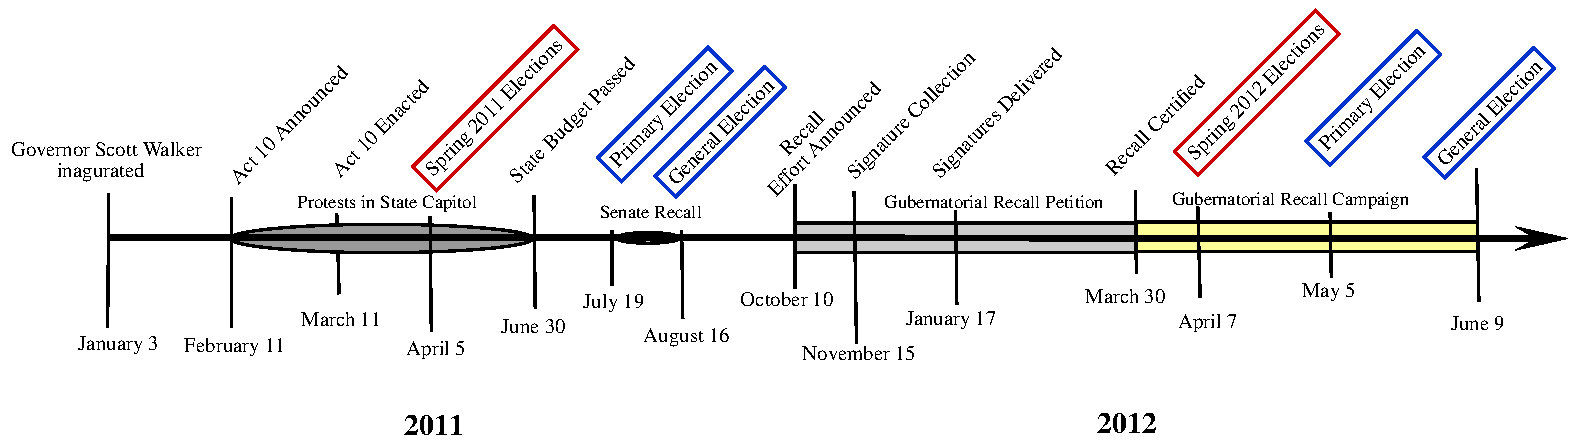
\includegraphics[width=\textwidth,height=1.75in]{img/wiscotimeline}
\end{figure}
\end{center}

\begin{center}
\begin{figure}[h!]
\begin{framed}
\caption{Budget Protests at the Wisconsin Capitol.  \copyright\ Justin Ormont | Wikimedia Commons | CC-BY-SA-3.0}
\label{fig:protest1}
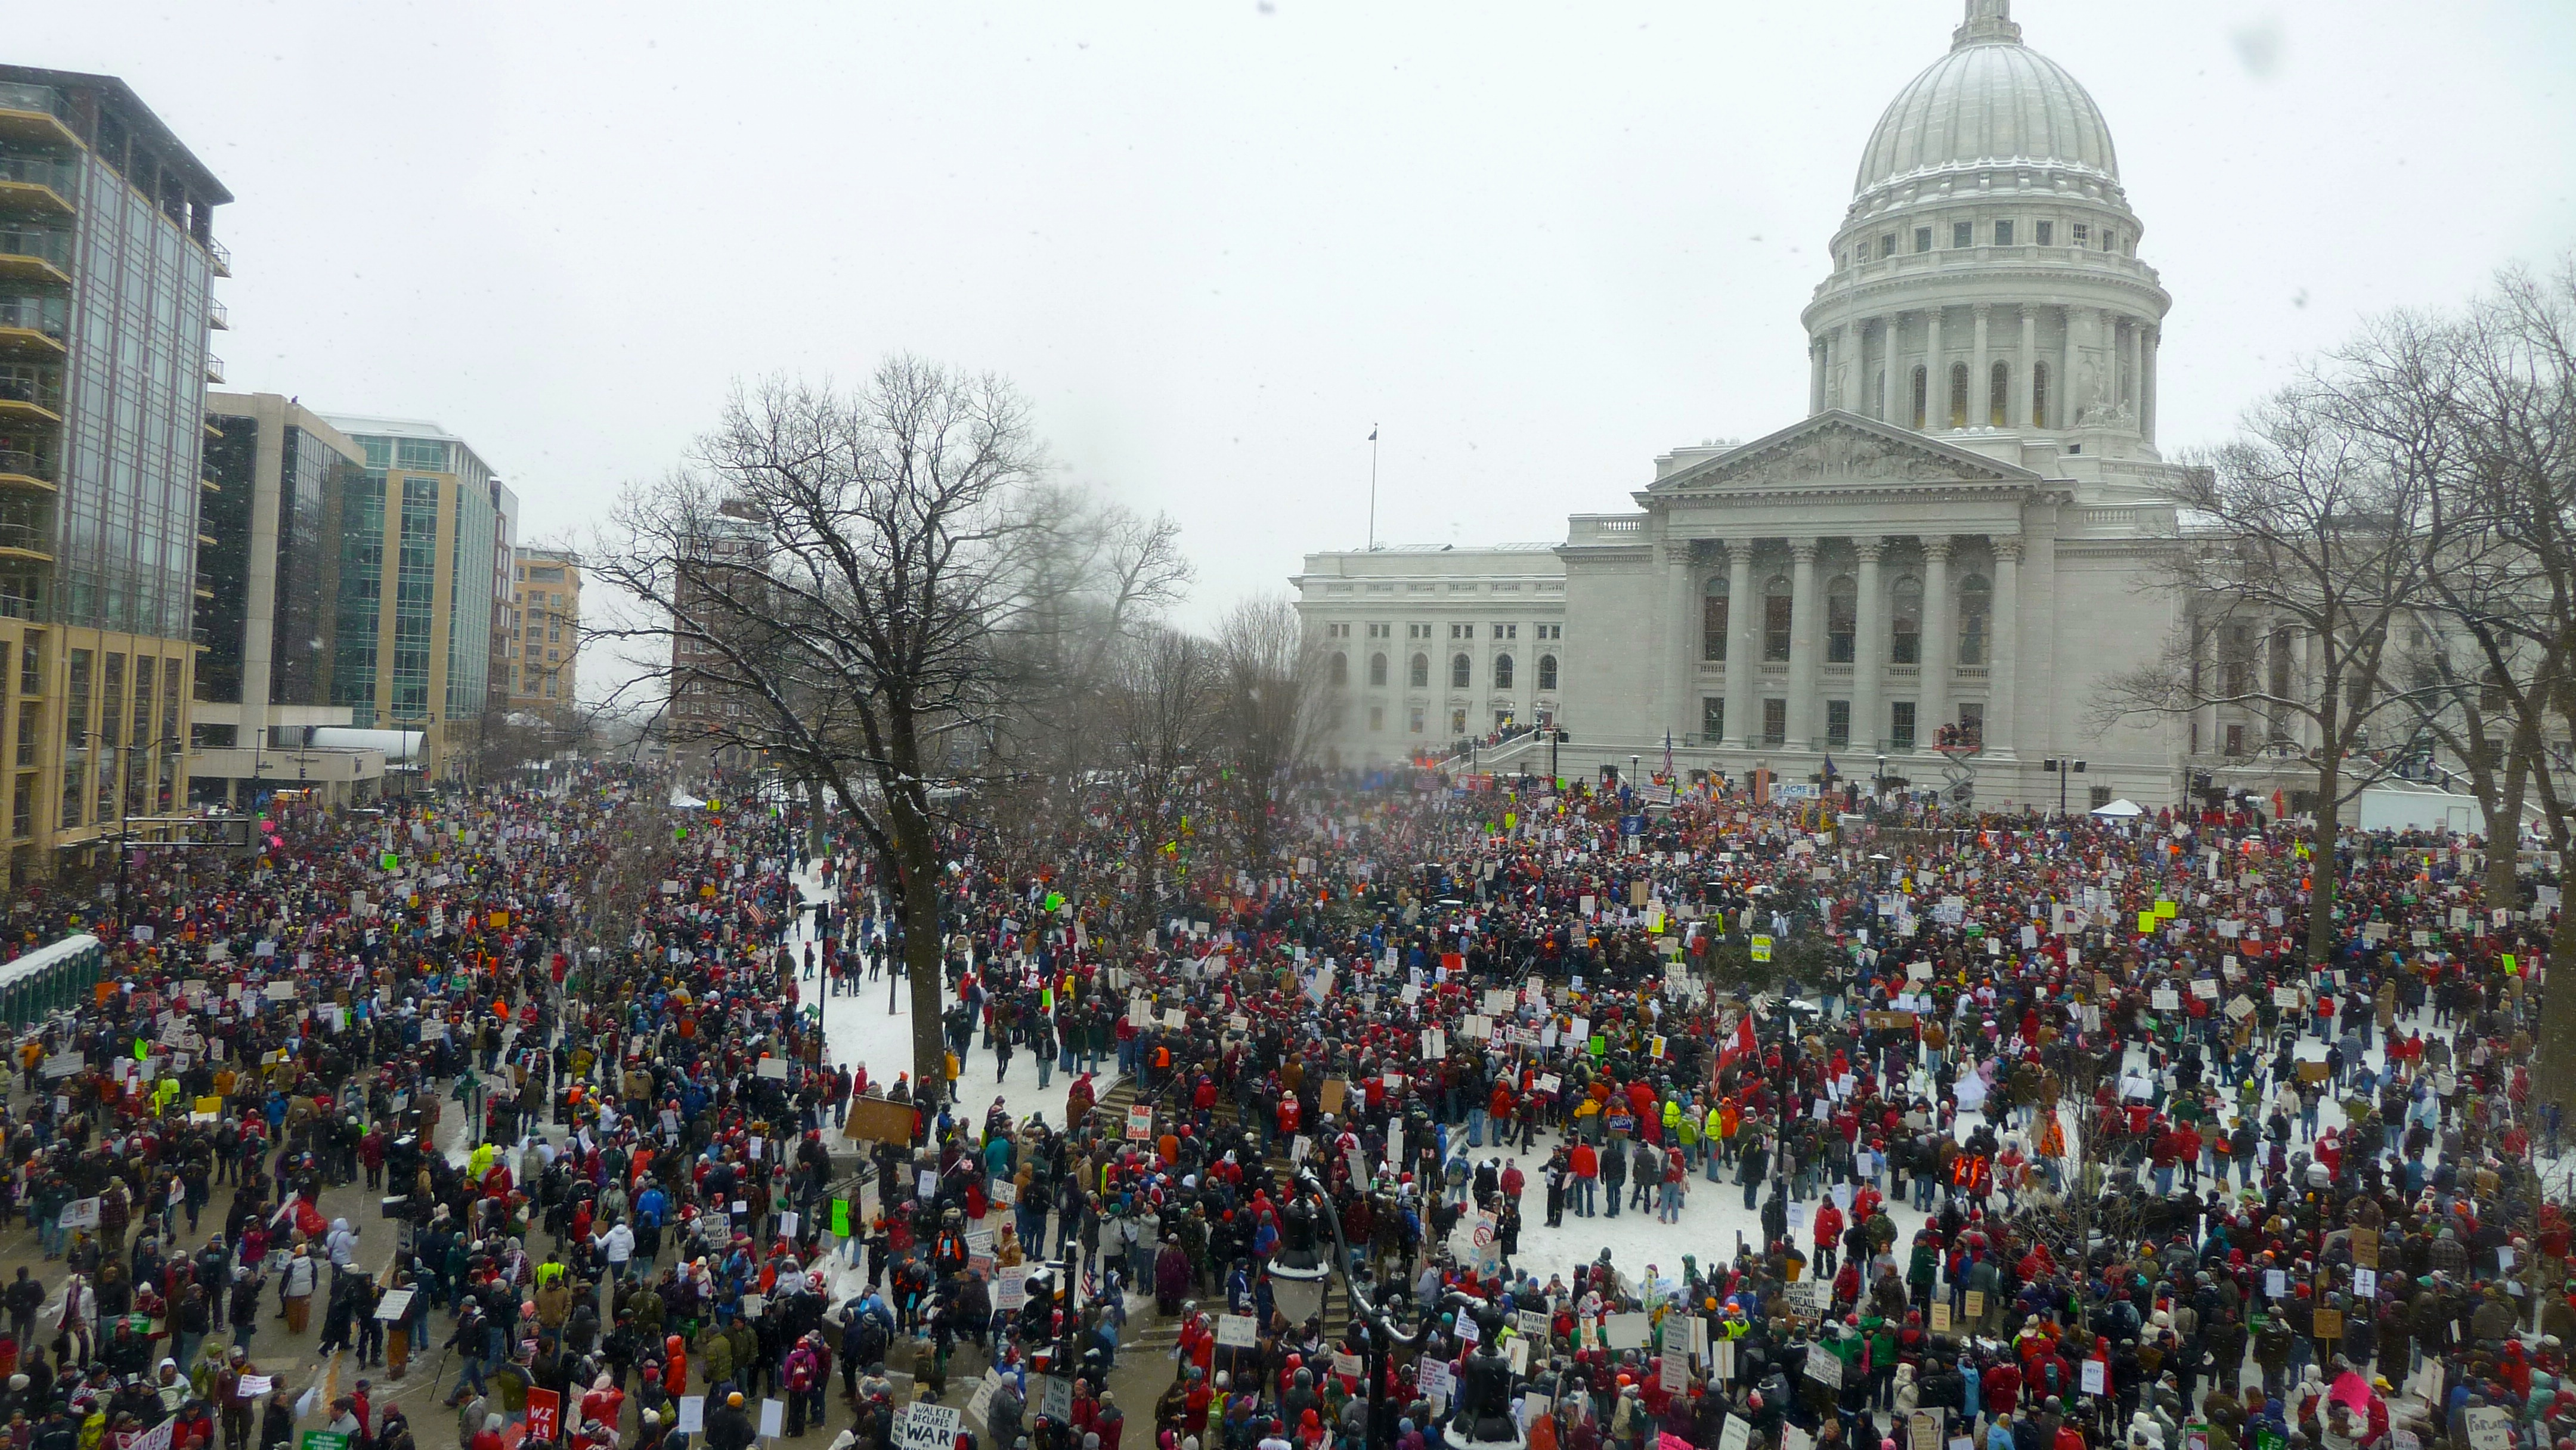
\includegraphics[width=4.425in,height=2.5in]{img/budgetProtest1}
\end{framed}
\end{figure}
\end{center}


\begin{center}
\begin{figure}[h!]
\begin{framed}
\caption{Budget Protests Inside the Capitol. \copyright\ Joe Rowley | Wikimedia Commons | CC-BY-SA-3.0 }
\label{fig:protest2}
\frame{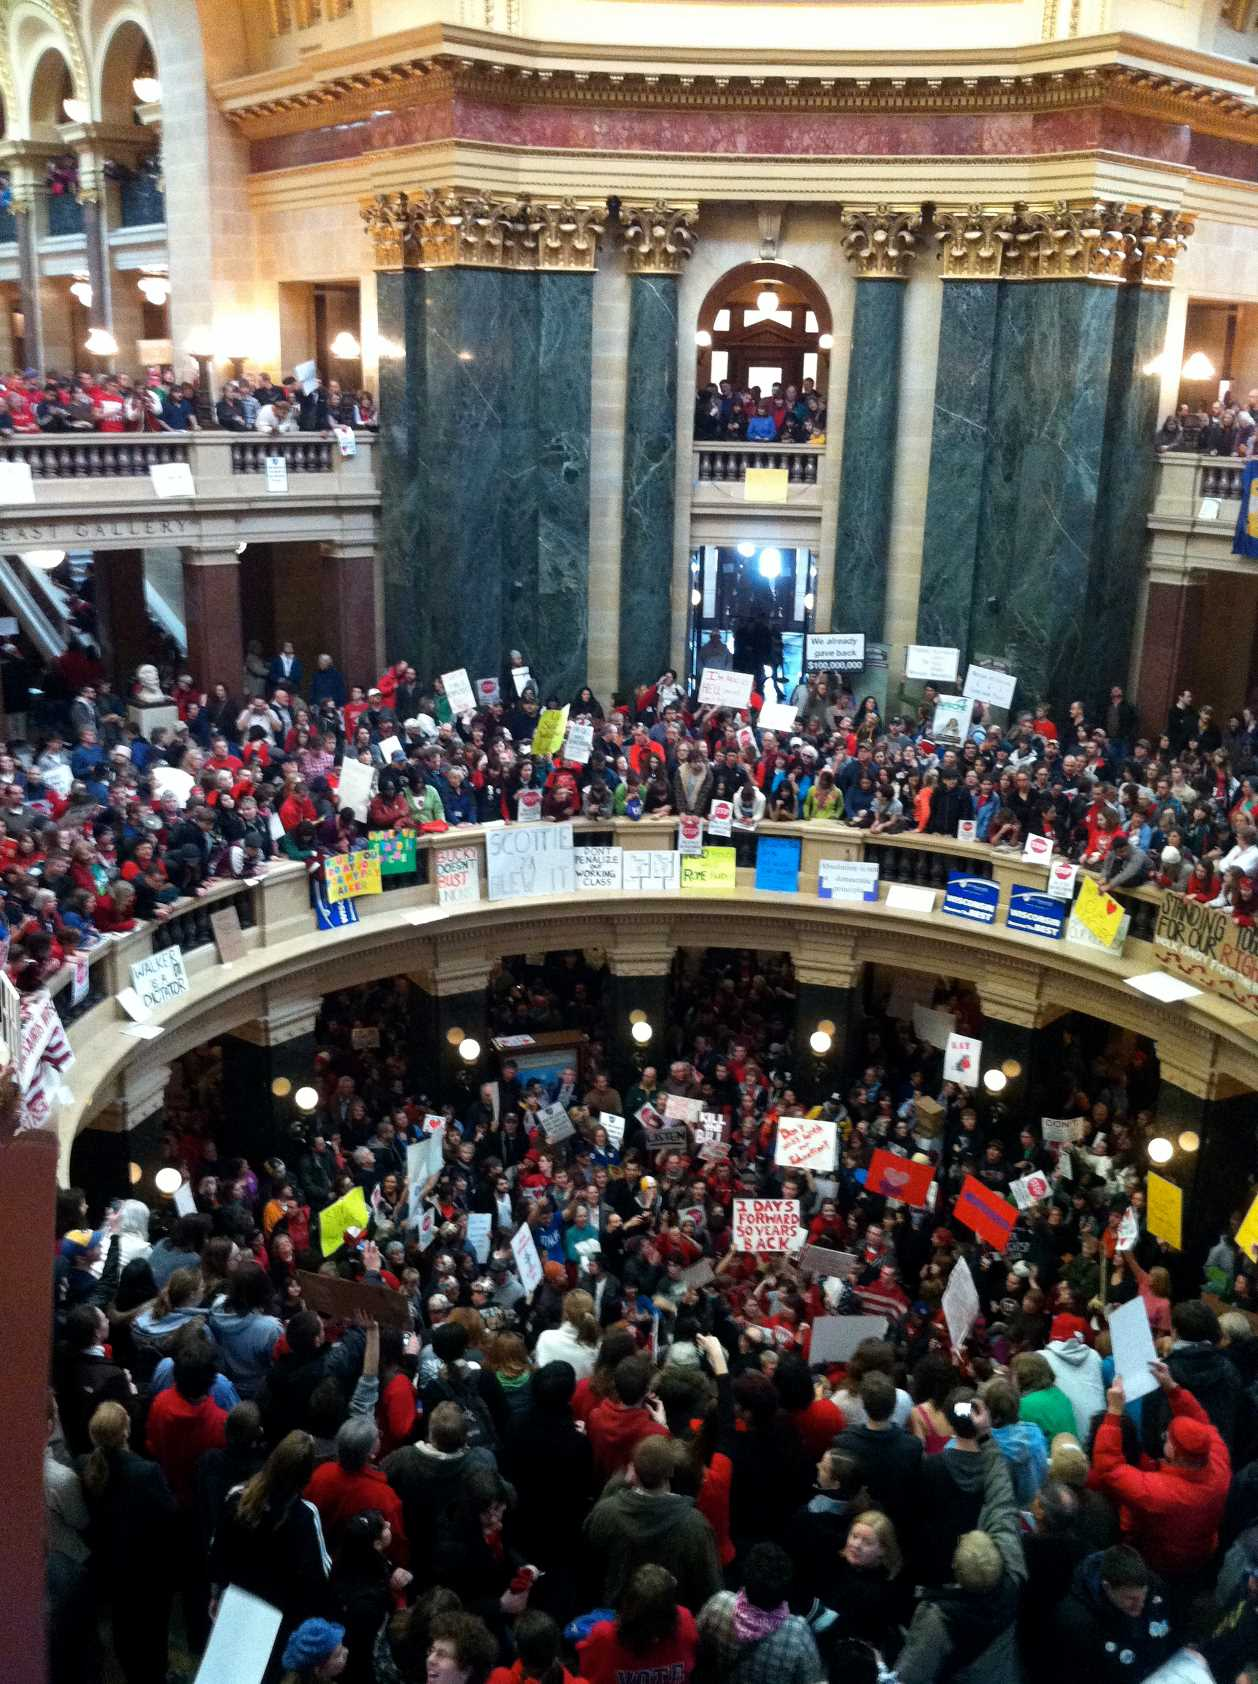
\includegraphics[width=3in,height=4in]{img/budgetProtest2}}
\end{framed}
\end{figure}
\end{center}

The new freedom to determine employee compensation outside of collectively bargained 
agreements meant that school boards now had more power. Importantly, 
this grant of power and increased political discourse surrounding the power of 
school boards relative to their employees was unanticipated by political observers 
and the public. It represents an exogenous shock because voters, school board 
members, and public employee unions had no knowledge prior to the introduction 
of the budget repair bill that the right to collectively bargain would be 
modified in 2011. \footnote{This last point is disputed by some conservative 
political observers and Scott Walker himself who claim that candidate Walker 
campaigned on this issue. However, the consensus has been that there is no record 
of any proposal during the 2010 campaign according to an investigation 
by the \href{http://www.politifact.com/wisconsin/statements/2011/feb/22/scott-walker/wisconsin-gov-scott-walker-says-he-campaigned-his-/}{Milwaukee Journal Sentinel}.} 

The events of 2011 and 2012 are depicted in Figure \ref{fig:wiscotimeline2}. Key 
events are marked as well as the dates of the spring school board elections of 
2011 and 2012. As Act 10's introduction was the precipitating event, I refer to 
this political unrest as the Act 10 period, which stretches from February 11, 2011 
with the introduction of Act 10 to Scott Walker's successful defeat of Milwaukee Tom 
Barrett in the recall election on June 9, 2012. I argue that the exogenous shock 
to the school board election process persists throughout this period because of 
the continual focus on education policy, school board politics, and the sustained 
polarization around Act 10 and Governor Walker's education policy. For example, 
after Act 10 was passed it became entangled in court battles while protestors 
turned their attention to the Wisconsin 2011-2013 Biennial Budget and its  
substantial cuts to school funding. Additionally, a signature drive for recall 
elections against several state senators was underway through the spring and 
summer. After that, the 2012 spring primary election took 
place during the heart of the recall petition signature drive and the spring 
2012 general eletions took place after the recall petition signatures were made public 
at the start of the gubernatorial recall election campaign. I conclude that this 
period then represented an unprecedented period of contention over the politics 
of school districts and education policy in Wisconsin. I argue that this Act 10
period galvanized the debate around education policy in Wisconsin in three 
distinct ways. 

First, it forced school board members and teachers' unions to show their hands 
to the public with respect to bargaining agreements. After Act 10 
boards were given the ability to unilaterally set compensation plans for their 
staff, which account for approximately 90\% of their annual operating costs.
\footnote{SOURCE}. This 
new power strongly incentivized both employee unions and property owners to express 
their policy preference for school district expenditures to mobilize both candidates 
and voters. School boards now, more than ever, had the chance to actualize the 
preferences of voters either to hold down property taxes, or to protect school 
staff from budget cuts. Additionally, many school boards had the option of renewing 
their union contracts between the time that Act 10 was passed and the time the 
law took effect -- effectively honoring their existing compensation and working 
condition agreements into the future. The option to extend contracts or to enact 
changes in the compensation plan was a high profile decision faced by some school 
boards in the post Act 10 period. 

The second effect Act 10 had on school board elections is that it injected a 
partisan dimension into traditionally non-partisan school board races. Candidates 
had to take a position on Act 10 publicly, aligning themselves 
unfairly or not, with either Governor Walker and the Republican party or the 
Democrats in opposition. Thus, voters and candidates who may have faced informational 
deficits in participating in school board elections previously could quickly signal 
to one another their policy goals using a public statement in favor of or condeming 
Act 10. 

The third effect of Act 10 was an intensified public discourse over the 
stewardship of public schools. This statewide political debate surrounding
around Act 10, the historic protests, and the recall election campaign all 
increased the amount of information voters had about school boards, school board 
powers, and the positions of their local school boards on issues such as Act 10, 
school funding, and budget priorities. Thus the informational advantage possessed 
by members of some interest groups prior to Act 10 evaporated. 


\subsection{Expectations}

How might an exogenous shock like the Act 10 period affect school board elections? 
For candidates, it raises the potential benefit and lowers the cost of running. 
Challengers to current board members can now capitalize on the 
increased public awareness about school funding and compensation plans to distinguish 
themselves from incumbents. Additionally, these candidates have more information 
about the likelihood of their success based on the preferences 
of the voters in their school district for Governor Walker -- both in the 2010 
Gubenatorial race and in the 2012 recall. 

For voters, the advantages are perhaps even more clear. Now voters have a high 
profile polarizing issue into which to divide candidates. This increases the 
information available for voters, decreasing the costs of voting. Additionally, 
if boards are given more power, voters have more reason to believe that their 
policy preferences can be actualized by electing a candidate more closely related 
to their preferences. 

If school board members were already representing the preferences of the majority 
of their community, and not a majority of the spring election electorate, then 
this increased information would result in potential increases to participation, 
but not a substantive change in representation. Voters may be more active because 
of an increased interest in voting in general -- an issue we will return to later -- 
but the results should be largely the same. However, continuous participation 
theory suggests that by expanding the electorate and revealing more information 
about the preferences of board members, voters should be more likely to participate 
and reject candidates who represent the interests of those who were participating 
prior to the Act 10 period. On average, prior to Act 10, boards should have been 
representing the preferences of the few continual participants in the electoral 
process, and post Act 10 the expansion of information should increase the size 
of the electorate and diversify the preferences enough to result in new choices 
for voters. 

For dissatisfaction theory the story is more nuanced. Depending on where a 
community is in the cycle of insular policymaking to public dissatisfaction 
much change may not happen. That is, the impact of the Act 10 period will be 
mediated by the prior electoral activity in the school district. Specifically, 
if the board has already been made reflective of the interests of the broader 
community through a prior period of local upheaval, then the Act 10 period should 
have little effect on board membership. However, if the board was previously 
insular and little information about its position relative to those of the community 
was known, then the Act 10 period should result in larger impacts in these 
communities. As dissatisfaction theory suggests that these realignments 
of school boards to community preferences are rare, I expect that on average 
the Act 10 period should lead to an overall increase in competition, incumbent 
defeat, and voter participation. 

\begin{center}
\begin{figure}[h!]
\caption{A Theoretical Model of School Board Policy Shock}
\label{fig:model}
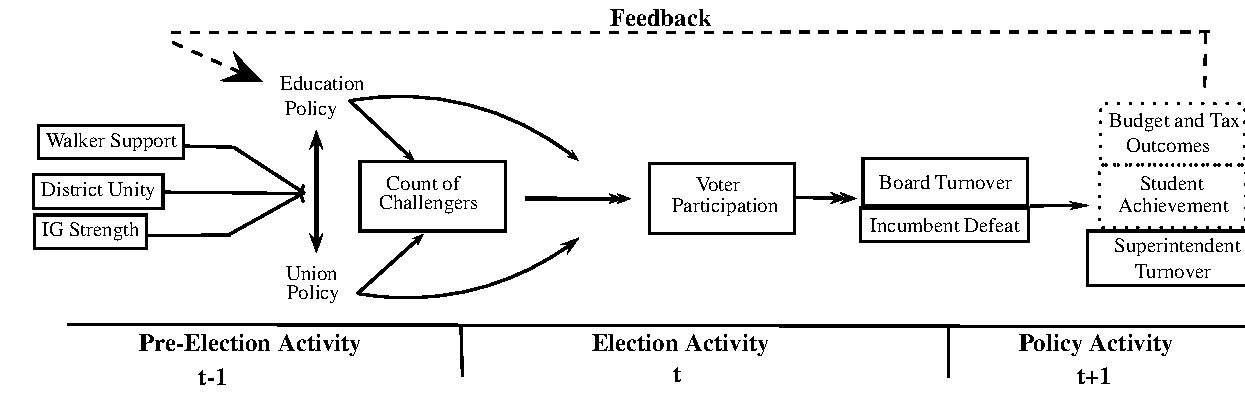
\includegraphics[width=.9\textwidth]{img/theory}
\end{figure}
\end{center}
\vspace{-24pt}

Figure \ref{fig:model} is reproduced from Chapter \ref{chap:intro}. It shows 
how preferences of the community and board policy in the pre-election period 
are related to the rise of challengers, voter participation, and incumbent defeat 
in the election period. Three potential indicators of the alignment of community 
and school board preferences are posited. The first is the level of support for 
Governor Walker's education policies in the Act 10 period. Second is the strength 
of support in the community for those preferences. Third is the relative strength 
of interest groups in the community -- specifically in this case teachers' 
unions. The next section describes these measures in more detail. 

To measure the impact on the actualized democracy in school districts, I use 
five separate measures of democratic activity. The first three are related 
measures of contestation. I use two categorizations of elections as either 
uncontested, ``minorly contested'', and ``seriously contested''. Races with 
challengers receiving 20 or more votes are considered ``seriously contested'', 
while races with at least a nominal challenger are considered ``minorly contested''. 
In addition to these categories, I employ a continuous measure of the 
competitiveness of a race that accounts for the number of seats available, number 
of voters casting ballots, and the number of votes necessary for at least one 
candidate to move from being a winner to a loser \citep{blaislago}. This measure 
is known as the Blais-Lago quotient and was also used in Chapters \ref{chap:candidacy} 
and \ref{chap:turnout}. Finally, I use two separate measures of voter turnout. 
The first captures the raw turnout for school board races out of the total voting 
age population of the school district. The second captures the proportion of voters 
who rolloff, or fail to cast a ballot for school board but voted in the spring 
election \citep{wattenberg00}. 

Table \ref{tab:act10hypo} summarizes the expected relationships between these 
variables. Shock refers to the main effect of the Act 10 period on the election activity in a school district, relative to its prior school board election 
activity. Both continuous participation and dissatisfaction theory have the same expectation. However, evidence for dissatisfaction theory comes from the expectation 
that the interaction of mediating factors and the policy shock should have 
an impact on some of the dependent variables. 


\begin{table}[h!]
\begin{center}
\begin{small}
\caption[Expected Effects of Act 10 Period and Mediating Factors on Actualized 
Democracy]{Expected effect of Act 10 shock and mediating factors on key measures 
of actualized democratic activity in school districts. Shock refers to elections 
during the Act 10 period, polarization refers to the community divide in support 
of Governor Walker, recall refers to the level of participation in the recall 
election, and IG refers to the strength of the teachers' union in the school 
district.}
\label{tab:act10hypo}
\begin{tabular}{| p{.16\textwidth} | p{.12\textwidth} | p{.12\textwidth} | 
 p{.12\textwidth} | p{.12\textwidth} | p{.12\textwidth} | p{.12\textwidth} |} \hline
variable & shock & shock x polarization & shock x recall & shock x IG & 
      polarization & IG strength \\ \hline
Cont. Race & + & + & null & - & null & - \\ \hline
Inc. Def.  & + & + & +    & - & +    & - \\ \hline 
Blais-Lago & + & + & null & + & +    & - \\ \hline
Turnout    & + & + & +    & - & null & - \\ \hline
Rolloff    & - & - & -    & - & null & + \\ \hline
\end{tabular}
\end{small}
\end{center}
\end{table}

For example, both dissatisfaction theory and continuous participation theory 
anticipate that the Act 10 period should result in increases in all electoral 
activity and a decrease in rolloff, or spring election voters who do not 
cast a ballot for school board. Dissatisfaction theory suggests that the impact 
of the shock is larger in communities with greater polarization around Governor 
Walker. However, if teacher union strength is high, the impact of the Act 10 
shock should be attenuated as unions work to protect incumbents, deter 
challengers, and keep races close relative to communities with weaker teachers' 
union strength. 

Turnout should increase in the Act 10 period, and should increase even more in 
communities divided in their support of Governor Walker.\footnote{One concern 
might be that the polarization was so extreme and the state so saturated with 
negative campaigning of all forms that voter turnout was suppressed even in the 
case of spring school board elections \citep{NegativeCamp1999}.} This matches 
studies of other elections by \citet{Lassen2005} who leveraged an exogenous shock 
of an information campaign in some electoral districts and found that 
increasing voters' information also produced a sizeable effect on the propensity 
to vote. However, if interest group activity is strong, in the pre-shock period 
we should see voter turnout be suppressed, but in the post-shock period we should 
see turnout increase as teachers' unions attempt to mobilize a show of force 
at the ballot box in support of their candidates locally. 

\subsection{Threats to Validity}

The argument above is not without its counterpoints. Critics might counter that 
though voters were mobilized in the Act 10 period, it had nothing to do with 
school boards. The 2011 spring election was also marked by a highly contested 
statewide Supreme Court election and the ultimate impact of Act 10 was in doubt 
due to multiple legal challenges. Voters in this period may have been motivated 
almost entirely by the statewide Supreme Court race and any participation in 
school board elections was purely incidental. By the 2012 spring election, Act 10 
was ruled as constitutional and there was no policy shock. Moreover, though Act 10 
now gave school boards more power, it came coupled with historical cuts in 
state aid and a freeze on school district revenue limits. In practice this 
meant that though compensation policy may have been freed up, school boards had 
very little flexibility to innovate under such fiscal constraint and school board 
office may have appeared particularly unappealing to potential candidates. 

I believe this study addresses these concerns in several ways. First, instead of 
focusing on a single measure of actualized democracy, I apply multiple measures. 
For example, while turnout may be subjected to political forces like statewide 
interest in a Supreme Court race, school board incumbent defeat and school board 
ballot rolloff are not. In addition to multiple outcome measures, I measure the 
policy shock of the Act 10 period as two distinct events, instead of averaging 
across the 2011 and 2012 elections. This has two benefits. First, it more closely 
reflects the reality that different conditions were in place in each election. 
More importantly, it allows for the effect of the Act 10 period to be measured 
with more nuance and the persistence of the effect to be explored. I also test 
for mediation effects. While it is not possible to measure and model all 
possible biasing omitted variables, I can search for some that theory suggests 
may explicitly be modifying the impact of the Act 10 period. For the rest, 
I can employ the panel nature of the data to focus on within district comparisons 
which difference out all time invariant unobservable characteristics. 

I now turn to describing the data and methods I employ to achieve this. 

\section{Data}

The data in this chapter is drawn from a unique collection of school board election 
results in Wisconsin school districts from 2002-2012. In addition to the election 
results from over 75\% of Wisconsin school districts, administrative records are 
incorporated to include annual measures of school districts on fiscal, political, 
demographic, and educational dimensions.

\subsection{Dependent Variables}

In this section I outline the key dependent variables for this investigation. 
Broadly, I am looking for evidence of the causal impact of the Act 10 period
on the behavior of both candidates and voters. For candidates, I look 
for a change in the patterns of candidate contestation and seat competitiveness 
after the passage of Act 10 and the granting of additional powers to school boards. 
For voters, I look for changes in voter turnout and decreases in voter rolloff. 

\begin{knitrout}
\definecolor{shadecolor}{rgb}{0.969, 0.969, 0.969}\color{fgcolor}\begin{figure}

\includegraphics[width=\maxwidth,height=3.18in]{../../phd_figs/chap6-blaisLagoplot-1} \caption[Lagged Competitiveness Across Years]{Lagged Competitiveness Across Years}\label{fig:blaisLagoplot}
\end{figure}


\end{knitrout}


% latex table generated in R 3.1.2 by xtable 1.7-4 package
% Mon Mar 02 21:23:05 2015
\begin{table}[ht]
\centering
\begin{tabular}{rrr}
  \hline
 & No Serious Contestation & Serious Contestation \\ 
  \hline
2007 & 188 & 108 \\ 
  2008 & 206 & 92 \\ 
  2009 & 200 & 96 \\ 
  2010 & 188 & 109 \\ 
  2011 & 195 & 108 \\ 
  2012 & 201 & 101 \\ 
   \hline
\end{tabular}
\caption{Frequency of Incumbency and Contestation.} 
\label{tab:serConyear}
\end{table}



Figure \ref{fig:blaisLagoplot} shows the relationship between lagged district 
competitiveness and district competitiveness changes slightly in 2011 and 2012 
from the global linear model represented by the dashed line. 
Table \ref{tab:serConyear} shows the number of districts with serious 
contestation for school board by year since 2006. The sample is relatively 
consistent over this period and there appears to be no change in the number 
of districts with seriously contested races across the years. 


Figures \ref{fig:turnoutPlot1} and \ref{fig:turnoutPlot2} show the relationship 
between school board turnout and voter rolloff and their respective lags. In 
2011 and 2012 the relationship deviates from the pooled across year relationship 
represented by the dashed line. In 2011 the slope looks the same, but the intercept 
is much higher suggesting higher overall turnout. In 2012, the slope is steeper, 
but the intercept is close to the same. This looks like a good argument for 
considering a twice lagged measure as the strange year to year relationships may 
be due to the cyclical nature of these elections. 

For rolloff, 2011 is clearly a standout year, while 2012 appears to fall right 
in line with the pooled across year relationship represented by the dashed line. 


\begin{knitrout}
\definecolor{shadecolor}{rgb}{0.969, 0.969, 0.969}\color{fgcolor}\begin{figure}

\includegraphics[width=\maxwidth,height=3.18in]{../../phd_figs/chap6-turnoutPlot1-1} \caption[Lagged School Board Turnout Across Years]{Lagged School Board Turnout Across Years}\label{fig:turnoutPlot1}
\end{figure}


\end{knitrout}

\begin{knitrout}
\definecolor{shadecolor}{rgb}{0.969, 0.969, 0.969}\color{fgcolor}\begin{figure}

\includegraphics[width=\maxwidth,height=3.18in]{../../phd_figs/chap6-turnoutPlot2-1} \caption[Lagged Spring Rolloff Across Years]{Lagged Spring Rolloff Across Years}\label{fig:turnoutPlot2}
\end{figure}


\end{knitrout}


\subsection{Independent Variables}

Figure \ref{fig:pairsPlot} shows the relationships among some key control variables 
and is similar to the plot introduced in Chapter \ref{chap:turnout}. These 
variables are related to the key independent variables identified by 
\citet{RefWorks:297} as indicators of school districts in transition from insular 
to competitive in their politics. 

\begin{knitrout}
\definecolor{shadecolor}{rgb}{0.969, 0.969, 0.969}\color{fgcolor}\begin{figure}

\includegraphics[width=\maxwidth]{../../phd_figs/chap6-pairsPlot-1} \caption[Pairs Plot of Demographic Variables and Turnout in 2012]{Pairs Plot of Demographic Variables and Turnout in 2012}\label{fig:pairsPlot}
\end{figure}


\end{knitrout}


\subsection{New Measures}

In addition to the suite of independent variables found in Chapters 
\ref{chap:candidacy} and \ref{chap:turnout}, this chapter features some additional 
key dependent variables drawn from results of Wisconsin's historic recall election. 
The Act 10 period itself created three unique measures available statewide to 
provide a window into the preferences of communities. First, the level of 
polarization in the community in the recall election of Scott Walker. The result 
of this election can be seen largely as an opinion poll of voters on the issues of 
Act 10 and education funding in the state -- the two largest issues in the 
campaign.\footnote{While some have argued that another issue, the legitimacy of
recalling the Governor in the first place was also important, this may also be a
reflection on how strongly those voters felt about Act 10 in the first place.} 

A second measure that arises from this period is the level of turnout for the 
recall election itself. As with any election, voters without a strong preference 
either way were able to stay home. What's more, the election was at an unconventional 
time -- neither during the fall or the spring general election. Turnout was 
specifically driven by a desire to express support or opposition to the Governor. 
As such, it can be seen as an indication of the intensity with which a community 
was in favor of or against the policies of the Governor. \footnote{The recall election 
took place on June $5^{th}$, 2012. Turnout was 57.4\% with 2,516,065 voters 
casting votes for Governor out of a voting age population of 4,378,741. For more 
information see \url{http://gab.wi.gov/sites/default/files/Statewide\%20Percentage\%20Results_6.5.12\%20Recall\%20Election\_PRE\%20SEN21\%20RECOUNT.pdf}}

A final measure was created by the mechanics of Act 10 itself. Act 10 required 
public employee unions to recertify through an election process. Over the next 
few years all public employee unions in Wisconsin held recertification elections. 
Recertification required unions to hold elections and that a majority of all 
members, not just of those who voted, must vote in favor of recertifying for 
the union to continue to operate. The results of these elections -- the margin 
by which the union recertified -- can be seen as a measure of latent union 
strength. While the vast majority of unions recertified, in many cases the 
elections were close.\footnote{Details on state law surrounding this.}

Each of these measures was made available \emph{after} the exogenous shock and 
as such can be considered to be \emph{post-treatment} variables. As I will argue 
below, I believe these measures can be interpreted as measuring latent traits 
within the communities and thus serve as \emph{pre-treatment} proxies of community 
traits which would not have been measured statewide without intervention. 

\subsubsection{Polarization}

Figure \ref{fig:ivPlot1} shows the relationship between recall polarization and 
other variables for the year 2012. THe relationship between fall and recall election 
turnout and polarization is virtually identical. The top right panel shows the 
relationship between recall polarization and the Democratic share of the most 
recent presidential two-party vote - aside from a handful of outliers it follows 
in the expected direction. Finally, spring election turnout is fairly similar to 
the other turnout variables, but at a lower level with about half the turnout 
on average of the other elections. 


\begin{knitrout}
\definecolor{shadecolor}{rgb}{0.969, 0.969, 0.969}\color{fgcolor}\begin{figure}

\includegraphics[width=\maxwidth]{../../phd_figs/chap6-ivPlot1-1} \caption[Polarization and Other Variables]{Polarization and Other Variables}\label{fig:ivPlot1}
\end{figure}


\end{knitrout}

Figure \ref{fig:ivPlot2} explores the relationship between recall polarization 
and demographic variables to understand the ways party-polarization in the recall 
is similar to or different than partisan polarization in other elections. In the 
top left there is a strong relationship between the logged median income and 
polarization with higher polarization more strongly associated with lower income. 
Polarization appears to be consistent across the size of the Voting Age Population 
(VAP). There is a slight increase in polarization as the percentage of VAP over 
65 increases. 

\begin{knitrout}
\definecolor{shadecolor}{rgb}{0.969, 0.969, 0.969}\color{fgcolor}\begin{figure}

\includegraphics[width=\maxwidth]{../../phd_figs/chap6-ivPlot2-1} \caption[Polarization and Population Control Variables]{Polarization and Population Control Variables}\label{fig:ivPlot2}
\end{figure}


\end{knitrout}

\subsubsection{WERC Elections}

The Act 10 period forced teachers' unions to show their strength through 
recertification elections. Statewide, most unions recertified sometime in the 
period from 2011-2013. While previously the proportion of the electorate composed 
of teachers was used as a proxy for teacher union strength in Chapter 
\ref{chap:turnout}, this measure is a measure of the cohesiveness and political
strength of teachers' unions. The Wisconsin Employment Relations Commission (WERC) maintains records of the annual recertification of unions. I use WERC records 
from each year following the passage of Act 10. After Act 10, unions in school
districts had to recertify in waves as their existing union contracts expired. 
I take WERC election results from 2011, 2012, 2013, and 2014. After recertifying 
the first time, unions must hold an annual recertification election. I collapse 
the recertifcation elections for all unions in the district available in all years 
as a measure of union strength over time. 

Turnout is a strong proxy for union strength because such vote records are public 
record. Teachers have little financial incentive to participate in the union 
post Act 10 as the union is barred legally from bargaining for anything other 
than an inflation indexed wage increase. 


Figure \ref{fig:ivPlot3} shows the relationship between independent variables and 
the turnout in school district union certification elections after the passage 
of Act 10. Polarization is slightly negatively related with WERC turnout. 
Median income is slightly positively related with WERC turnout. VAP and \% of 
VAP over 65 are not really related to this. 

\begin{knitrout}
\definecolor{shadecolor}{rgb}{0.969, 0.969, 0.969}\color{fgcolor}\begin{figure}

\includegraphics[width=\maxwidth]{../../phd_figs/chap6-ivPlot3-1} \caption[Polarization and WERC Elections]{Polarization and WERC Elections}\label{fig:ivPlot3}
\end{figure}


\end{knitrout}


\clearpage



\section{Methods}

I now describe the models fit to the data and how to understand parameters.  

\subsection{Causal Inference}

Extraordinary claims require extraordinary evidence, and there is no more 
extraordinary claim a quantitative analyst can make than causality from 
observational data. To credibly claim that the estimate of the effect of Act 10 
and the power granted to school boards, I must demonstrate both how this impact 
is exogenous and how I will operationalize it into a variable. Above, I have 
already described how the events surrounding the passage of Act 10 were 
unforeseen by the electorate and therefore not endogenous to school board 
elections post Act 10. 

To operationalize this exogenous shock I code all observations that occur after 
the passage of Act 10 as having a treatment condition of 1, and all of those 
observations in periods before Act 10 as having a treatment condition of 0. If 
this was a randomized experiment and exposure to Act 10 had been randomly 
distributed to school districts and years, I could stop and simply compute 
the average levels of the dependent variables for these two groups and perform 
a t-test. However, as the prior chapters have shown, there exist substantial observable characteristics that affect candidate and voter participation. Not 
taking these variables into account risks allowing them to confound the 
estimation of the treatment effect and bias estimates away from the true 
impact \cite{gelhill}. 

Though school districts in Wisconsin were not randomly assigned to greater power 
and more engaged voters at different time periods, they were all assigned to this 
treatment at exactly the same moment with perfect fidelity. This eliminates one 
potential bias to estimating the causal impact of the treatment -- assignment 
bias. Now, by comparing districts to themselves pre and post assignment, we can 
be more sure that we are picking up the impact of the treatment. 

\subsection{Modeling Strategy}

I use multiple methods to triangulate the causal impact under different 
identifying assumptions. Leveraging the panel nature of my data, I can use 
two different methods to control for unobservable characteristics in the 
data. Using a lagged dependent variable I can control for time-variant 
unobservables that have the potential to bias causal estimates. Using unit 
fixed effects, for school districts, I can control for time-invariant 
unobservable characteristics. \citet{mhecon} demonstrate how under certain 
assumptions a lagged dependent variable and an individual fixed effect model 
can serve as a lower and upper bounds on the causal effect respectively. 

However, I still need to control for the effects that lead to variation in 
participation from election to election that are observable. To do this, 
and to make comparisons within districts, I employ a fixed effect strategy.
The equation below depicts this approach with the \emph{i}'s representing 
individual observations and the \emph{j}'s representing the individual 
districts in the sample. $\lambda$ represents the conditional estimate 
of the treatment, taking into account the within district variation and 
conditional on the control variables in $X_{ij}$. 

\begin{align*} 
y_{it} &= \alpha + \gamma_{i} + \beta X_{it} + \lambda T_{it} + \epsilon_{it}  \\ 
\end{align*}


\subsection{Threats to Validity}

Claims of causality rest on assumptions. In addition to the assumption that the 
passage of Act 10 was exogenous, unforeseen, and universal, this approach also 
assumes that all confounding covariates are observable and included in the model 
and that no omitted variables may bias the estimation of the treatment effect 
\cite{gelhill}. In practice, this assumption is not empirically verifiable. I 
argue that instead that the treatment effect is a valid estimate given the 
inclusion of terms to capture within district variance, a lagged 
dependent variable, and substantively important predictors of 
each of the dependent variables as demonstrated in previous chapters. 

% Citations: Shadish and Cook


% TODO: Describe a lagged observational model
% TODO: Difference in difference strategy
% TODO: Interrupted time series with district random effects


\section{Results}

I organize the results as follows. In the first section, I review the results 
for the models that leverage the years 2011 and 2012 as treated by a causal 
shock and I fit lagged time models and differences-in-differences estimates 
of the impact of Act 10 across five distinct measures of actualized democracy -- 
contestation, competitiveness, incumbent defeat, voter turnout, and voter 
rolloff. In the next section, I then step away from the causal framework and 
fit longitudinal models which seek to explore evidence, if any, that this causal 
impact was mediated. 

\subsection{Causal Estimates}

I provide three sets of results for each dependent variable. The first is a 
regression with a lagged dependent variable and demographic controls, the second 
is a differences in differences estimate, and the third is a difference in 
differences estimate with district level random effects.\footnote{I tested the 
models on a restricted sample with only years after 2007, but this had no 
substantive impact on the results.}

%tab:causMinorCon



%tab:causSerCon
\begin{small}
\begin{table}[!ht]
\caption{Causal Estimates of Act 10 Period on Contestation}
\label{tab:causBL} 
\begin{tabular}{ l D{.}{.}{3}D{.}{.}{3}D{.}{.}{3} } 
\hline 
  & \multicolumn{ 1 }{ c }{ Lag } & \multicolumn{ 1 }{ c }{ DnD } & \multicolumn{ 1 }{ c }{ FE } \\ \hline
 %                                & Lag           & DnD           & FE           \\ 
(Intercept)                      & -4.737        & -4.742        & 0.220        \\ 
                                 & (3.113)       & (3.113)       & (0.261)      \\ 
contestSer\_lag1                & 0.638 ^{***}  & 0.632 ^{***}  &              \\ 
                                 & (0.111)       & (0.123)       &              \\ 
treatmentDiff1                   & -0.018        & -0.046        & -0.143       \\ 
                                 & (0.138)       & (0.174)       & (0.186)      \\ 
treatmentDiff2                   & -0.130        & -0.121        & -0.262       \\ 
                                 & (0.140)       & (0.186)       & (0.192)      \\ 
VAP\_adjLOG\_sq\_lag          & 0.003         & 0.003         &              \\ 
                                 & (0.045)       & (0.045)       &              \\ 
incumShare\_lag                 & -0.044        & -0.044        & 0.126        \\ 
                                 & (0.160)       & (0.160)       & (0.200)      \\ 
VAP\_adjLOG\_lag               & 0.432         & 0.434         &              \\ 
                                 & (0.787)       & (0.787)       &              \\ 
per65o\_lag                     & 1.317         & 1.321         &              \\ 
                                 & (1.741)       & (1.744)       &              \\ 
nraces\_lag                     & -0.137        & -0.136        & -0.172       \\ 
                                 & (0.098)       & (0.098)       & (0.207)      \\ 
OOH\_share\_lag                & 0.180         & 0.180         &              \\ 
                                 & (0.572)       & (0.573)       &              \\ 
PerBachelorOrAbove\_lag         & -2.776 ^{***} & -2.772 ^{***} &              \\ 
                                 & (0.819)       & (0.819)       &              \\ 
locale2\_lagexurb               & 0.143         & 0.141         &              \\ 
                                 & (0.464)       & (0.464)       &              \\ 
locale2\_lagrural               & 0.237         & 0.235         &              \\ 
                                 & (0.473)       & (0.473)       &              \\ 
contestSer\_lag1:treatmentDiff1 &               & 0.075         &              \\ 
                                 &               & (0.286)       &              \\ 
contestSer\_lag1:treatmentDiff2 &               & -0.022        &              \\ 
                                 &               & (0.284)       &               \\
 $N$                              & 2354          & 2354          & 2354         \\ 
AIC                              & 2940.110      & 2944.027      & 2942.868     \\ 
BIC                              & 3239.831      & 3289.859      & 10090.068    \\ 
$\log L$                        & -1418.055     & -1412.013     & -231.434      \\ \hline
 \multicolumn{4}{l}{\footnotesize{$^\dagger$ significant at $p<.10$; $^* p<.05$; $^{**} p<.01$; $^{***} p<.001$}}\\
\multicolumn{4}{l}{\footnotesize{Fixed effect model includes district fixed effects - not reported.}} 
\end{tabular} 
 \end{table}

\end{small}

%tab:causBL
\begin{small}
\begin{table}[!ht]
\caption{Causal Estimates of Act 10 Period on Competitiveness}
\label{tab:causBL} 
\begin{tabular}{ l D{.}{.}{3}D{.}{.}{3}D{.}{.}{3} } 
\hline 
  & \multicolumn{ 1 }{ c }{ Lag } & \multicolumn{ 1 }{ c }{ DnD } & \multicolumn{ 1 }{ c }{ FE } \\ \hline
 %                                 & Lag               & DnD               & FE               \\ 
(Intercept)                       & 5.450 ^*          & 5.448 ^*          & 1.221 ^{***}     \\ 
                                  & (2.234)           & (2.223)           & (0.138)          \\ 
minBlaisLago\_lag                & 0.151 ^{***}      & 0.129 ^{***}      &                  \\ 
                                  & (0.027)           & (0.028)           &                  \\ 
treatmentDiff1                    & 0.116             & -0.012            & 0.181            \\ 
                                  & (0.107)           & (0.176)           & (0.111)          \\ 
treatmentDiff2                    & -0.013            & -0.267 ^\dagger  & 0.026            \\ 
                                  & (0.103)           & (0.161)           & (0.110)          \\ 
VAP\_adjLOG\_sq\_lag           & 0.011             & 0.011             &                  \\ 
                                  & (0.034)           & (0.034)           &                  \\ 
incumShare\_lag                  & -0.052            & -0.053            & -0.213 ^\dagger \\ 
                                  & (0.122)           & (0.122)           & (0.120)          \\ 
VAP\_adjLOG\_lag                & -0.679            & -0.670            &                  \\ 
                                  & (0.567)           & (0.564)           &                  \\ 
per65o\_lag                      & -0.144            & -0.161            &                  \\ 
                                  & (1.410)           & (1.402)           &                  \\ 
nraces\_lag                      & 0.766 ^{***}      & 0.767 ^{***}      & 0.135            \\ 
                                  & (0.076)           & (0.076)           & (0.109)          \\ 
OOH\_share\_lag                 & -0.263            & -0.278            &                  \\ 
                                  & (0.462)           & (0.460)           &                  \\ 
PerBachelorOrAbove\_lag          & 2.905 ^{***}      & 2.925 ^{***}      &                  \\ 
                                  & (0.670)           & (0.663)           &                  \\ 
locale2\_lagexurb                & 0.202             & 0.203             &                  \\ 
                                  & (0.366)           & (0.365)           &                  \\ 
locale2\_lagrural                & 0.120             & 0.125             &                  \\ 
                                  & (0.349)           & (0.349)           &                  \\ 
minBlaisLago\_lag:treatmentDiff1 &                   & 0.064             &                  \\ 
                                  &                   & (0.060)           &                  \\ 
minBlaisLago\_lag:treatmentDiff2 &                   & 0.130 ^*          &                  \\ 
                                  &                   & (0.059)           &                   \\
 $N$                               & 2354              & 2354              & 2354             \\ 
$R^2$                             & 0.170             & 0.172             & 0.401            \\ 
adj. $R^2$                        & 0.165             & 0.167             & 0.310            \\ 
Resid. sd                         & 1.690             & 1.689             & 1.536             \\ \hline
 \multicolumn{4}{l}{\footnotesize{$^\dagger$ significant at $p<.10$; $^* p<.05$; $^{**} p<.01$; $^{***} p<.001$}}\\
\multicolumn{4}{l}{\footnotesize{Fixed effect model includes district fixed effects - not reported.}} 
\end{tabular} 
 \end{table}

\end{small}

%tab:causID
\begin{small}
\begin{table}[!ht]
\caption{Causal Estimates of Act 10 Period on Incumbent Defeat}
\label{tab:causID} 
\begin{tabular}{ l D{.}{.}{3}D{.}{.}{3}D{.}{.}{3} } 
\hline 
  & \multicolumn{ 1 }{ c }{ Lag } & \multicolumn{ 1 }{ c }{ DnD } & \multicolumn{ 1 }{ c }{ FE } \\ \hline
 %                               & Lag               & DnD               & FE               \\ 
(Intercept)                     & -8.272 ^*         & -8.298 ^*         & -19.309 ^{***}   \\ 
                                & (3.417)           & (3.431)           & (1.128)          \\ 
incDefeats\_lag                & 0.358 ^{**}       & 0.410 ^{**}       &                  \\ 
                                & (0.139)           & (0.153)           &                  \\ 
treatmentDiff1                  & -0.345 ^\dagger  & -0.267            & -0.385 ^\dagger \\ 
                                & (0.182)           & (0.193)           & (0.223)          \\ 
treatmentDiff2                  & 0.028             & 0.060             & 0.038            \\ 
                                & (0.170)           & (0.196)           & (0.212)          \\ 
VAP\_adjLOG\_sq\_lag         & -0.068            & -0.068            &                  \\ 
                                & (0.049)           & (0.049)           &                  \\ 
VAP\_adjLOG\_lag              & 1.458 ^\dagger   & 1.464 ^\dagger   &                  \\ 
                                & (0.847)           & (0.852)           &                  \\ 
per65o\_lag                    & 0.036             & -0.018            &                  \\ 
                                & (2.071)           & (2.075)           &                  \\ 
nraces\_lag                    & -0.119            & -0.120            & -0.173           \\ 
                                & (0.129)           & (0.129)           & (0.282)          \\ 
OOH\_share\_lag               & -0.031            & -0.045            &                  \\ 
                                & (0.695)           & (0.694)           &                  \\ 
PerBachelorOrAbove\_lag        & -3.282 ^{**}      & -3.307 ^{**}      &                  \\ 
                                & (1.034)           & (1.038)           &                  \\ 
incumShare\_lag                & -0.205            & -0.207            & -0.013           \\ 
                                & (0.172)           & (0.173)           & (0.238)          \\ 
locale2\_lagexurb              & 0.146             & 0.148             &                  \\ 
                                & (0.383)           & (0.386)           &                  \\ 
locale2\_lagrural              & -0.070            & -0.068            &                  \\ 
                                & (0.421)           & (0.423)           &                  \\ 
incDefeats\_lag:treatmentDiff1 &                   & -0.438            &                  \\ 
                                &                   & (0.506)           &                  \\ 
incDefeats\_lag:treatmentDiff2 &                   & -0.129            &                  \\ 
                                &                   & (0.388)           &                   \\
 $N$                             & 2354              & 2354              & 2354             \\ 
AIC                             & 2192.218          & 2195.367          & 2392.015         \\ 
BIC                             & 2491.939          & 2541.200          & 9539.216         \\ 
$\log L$                       & -1044.109         & -1037.684         & 43.992            \\ \hline
 \multicolumn{4}{l}{\footnotesize{$^\dagger$ significant at $p<.10$; $^* p<.05$; $^{**} p<.01$; $^{***} p<.001$}}\\
\multicolumn{4}{l}{\footnotesize{Fixed effect model includes district fixed effects - not reported.}} 
\end{tabular} 
 \end{table}

\end{small}

%tab:causTurn
\begin{small}
\begin{table}[!ht]
\caption{Causal Estimates of Act 10 Period on Turnout}
\label{tab:causTurn} 
\begin{tabular}{ l D{.}{.}{3}D{.}{.}{3}D{.}{.}{3} } 
\hline 
  & \multicolumn{ 1 }{ c }{ Lag } & \multicolumn{ 1 }{ c }{ DnD } & \multicolumn{ 1 }{ c }{ FE } \\ \hline
 %                            & Lag           & DnD           & FE           \\ 
(Intercept)                  & -1.615        & -1.641        & -1.915 ^{***}\\ 
                             & (1.400)       & (1.410)       & (0.190)      \\ 
turnout\_lag                & 0.216 ^{***}  & 0.253 ^{***}  &              \\ 
                             & (0.026)       & (0.031)       &              \\ 
treatmentDiff1               & 0.529 ^{***}  & 0.367 ^{**}   & 0.556 ^{***} \\ 
                             & (0.022)       & (0.119)       & (0.022)      \\ 
treatmentDiff2               & 0.292 ^{***}  & -0.082        & 0.253 ^{***} \\ 
                             & (0.027)       & (0.097)       & (0.025)      \\ 
VAP\_adjLOG\_sq\_lag      & 0.014         & 0.013         &              \\ 
                             & (0.013)       & (0.014)       &              \\ 
VAP\_adjLOG\_lag           & -0.347        & -0.337        &              \\ 
                             & (0.225)       & (0.232)       &              \\ 
per65o\_lag                 & 1.590 ^{***}  & 1.547 ^{***}  &              \\ 
                             & (0.441)       & (0.443)       &              \\ 
nraces\_lag                 & -0.016        & -0.014        & -0.022       \\ 
                             & (0.020)       & (0.020)       & (0.056)      \\ 
OOH\_share\_lag            & -0.113        & -0.114        &              \\ 
                             & (0.156)       & (0.157)       &              \\ 
median\_incomeLOG\_lag     & 0.155         & 0.161         &              \\ 
                             & (0.111)       & (0.111)       &              \\ 
ImputedFlagYes               & -0.403 ^{***} & -0.399 ^{***} & -0.361 ^{***}\\ 
                             & (0.051)       & (0.052)       & (0.056)      \\ 
locale2\_lagexurb           & -0.075        & -0.075        &              \\ 
                             & (0.075)       & (0.076)       &              \\ 
locale2\_lagrural           & -0.026        & -0.024        &              \\ 
                             & (0.080)       & (0.082)       &              \\ 
PerBachelorOrAbove\_lag     & 0.340         & 0.332         &              \\ 
                             & (0.306)       & (0.308)       &              \\ 
fallTurnout\_lag            & 0.495 ^{**}   & 0.477 ^{**}   & 0.120        \\ 
                             & (0.175)       & (0.176)       & (0.214)      \\ 
turnout\_lag:treatmentDiff1 &               & -0.088        &              \\ 
                             &               & (0.065)       &              \\ 
turnout\_lag:treatmentDiff2 &               & -0.180 ^{***} &              \\ 
                             &               & (0.044)       &               \\
 $N$                          & 2325          & 2325          & 2325         \\ 
$R^2$                        & 0.320         & 0.324         & 0.501        \\ 
adj. $R^2$                   & 0.316         & 0.319         & 0.425        \\ 
Resid. sd                    & 0.421         & 0.420         & 0.386         \\ \hline
 \multicolumn{4}{l}{\footnotesize{$^\dagger$ significant at $p<.10$; $^* p<.05$; $^{**} p<.01$; $^{***} p<.001$}}\\
\multicolumn{4}{l}{\footnotesize{Fixed effect model includes district fixed effects - not reported.}} 
\end{tabular} 
 \end{table}

\end{small}

%tab:causRoll
\begin{small}
\begin{table}[!ht]
\caption{Causal Estimates of Act 10 Period on Rolloff}
\label{tab:causRoll} 
\begin{tabular}{ l D{.}{.}{3}D{.}{.}{3}D{.}{.}{3} } 
\hline 
  & \multicolumn{ 1 }{ c }{ Lag } & \multicolumn{ 1 }{ c }{ DnD } & \multicolumn{ 1 }{ c }{ FE } \\ \hline
 %                                & Lag               & DnD               & FE               \\ 
(Intercept)                      & -0.234            & -0.144            & 0.040            \\ 
                                 & (0.185)           & (0.178)           & (0.099)          \\ 
turnoutDiff\_lag                & 0.262 ^{***}      & 0.273 ^{***}      &                  \\ 
                                 & (0.065)           & (0.062)           &                  \\ 
treatmentDiff1                   & 0.055 ^{***}      & 0.039 ^{***}      & 0.056 ^{***}     \\ 
                                 & (0.005)           & (0.007)           & (0.005)          \\ 
treatmentDiff2                   & 0.037 ^{***}      & 0.039 ^{***}      & 0.033 ^{***}     \\ 
                                 & (0.005)           & (0.005)           & (0.005)          \\ 
VAP\_adjLOG\_sq\_lag          & -0.004 ^*         & -0.003 ^\dagger  &                  \\ 
                                 & (0.002)           & (0.002)           &                  \\ 
VAP\_adjLOG\_lag               & 0.081 ^*          & 0.069 ^*          &                  \\ 
                                 & (0.033)           & (0.033)           &                  \\ 
per65o\_lag                     & -0.006            & 0.006             &                  \\ 
                                 & (0.072)           & (0.068)           &                  \\ 
nraces\_lag                     & 0.002             & 0.001             & 0.008            \\ 
                                 & (0.003)           & (0.003)           & (0.008)          \\ 
OOH\_share\_lag                & 0.037             & 0.030             &                  \\ 
                                 & (0.033)           & (0.032)           &                  \\ 
median\_incomeLOG\_lag         & -0.027            & -0.028 ^\dagger  &                  \\ 
                                 & (0.017)           & (0.016)           &                  \\ 
ImputedFlagYes                   & 0.028 ^{**}       & 0.027 ^{**}       & 0.024 ^*         \\ 
                                 & (0.010)           & (0.010)           & (0.012)          \\ 
locale2\_lagexurb               & -0.014            & -0.012            &                  \\ 
                                 & (0.010)           & (0.010)           &                  \\ 
locale2\_lagrural               & -0.005            & -0.006            &                  \\ 
                                 & (0.010)           & (0.009)           &                  \\ 
PerBachelorOrAbove\_lag         & -0.070            & -0.049            &                  \\ 
                                 & (0.058)           & (0.055)           &                  \\ 
fallTurnout\_lag                & 0.146 ^{***}      & 0.133 ^{***}      & 0.102            \\ 
                                 & (0.038)           & (0.036)           & (0.118)          \\ 
turnoutDiff\_lag:treatmentDiff1 &                   & 0.446 ^{***}      &                  \\ 
                                 &                   & (0.115)           &                  \\ 
turnoutDiff\_lag:treatmentDiff2 &                   & -0.229 ^{**}      &                  \\ 
                                 &                   & (0.077)           &                   \\
 $N$                              & 1132              & 1132              & 1132             \\ 
$R^2$                            & 0.236             & 0.272             & 0.550            \\ 
adj. $R^2$                       & 0.226             & 0.262             & 0.387            \\ 
Resid. sd                        & 0.062             & 0.061             & 0.056             \\ \hline
 \multicolumn{4}{l}{\footnotesize{$^\dagger$ significant at $p<.10$; $^* p<.05$; $^{**} p<.01$; $^{***} p<.001$}}\\
\multicolumn{4}{l}{\footnotesize{Fixed effect model includes district fixed effects - not reported.}} 
\end{tabular} 
 \end{table}

\end{small}

\begin{table}[h!]
\begin{center}
\begin{small}
\caption{Summary of Causal Relationship of Act 10 Reforms on Board Elections}
\label{tab:act10resSummary}
\begin{tabular}{| p{.24\textwidth} | p{.12\textwidth} | p{.12\textwidth} | 
      p{.4\textwidth} |} \hline
DV / Variable & expected & observed & evidence \\ \hline
Contested Race & + & - & no statistical significance, wrong sign \\ \hline
Contesed Race (ser) & + & - & no statistical significance, wrong sign \\ \hline
Incumbent Defeat & + & - & weakly negative, weak statistical significance, only one year\\ \hline 
Competitiveness & + & +  & weakly positive, statistically significant for one year in 
diff in diff, not for FE\\ \hline
Turnout & + & + & diff in diff weakly negative, overall effect positive in both 
years \\ \hline
Rolloff & - & + & decrease in year 2, but incorrect sign, statistical significance 
in FE models\\ \hline
\end{tabular}
\end{small}
\end{center}
\end{table}

Table \ref{tab:act10resSummary} summarizes the results in comparison to the 
expectations from Table \ref{tab:act10hypo}. Overall, there is some evidence 
of an effect of Act 10 on school board election activity. Specifically, the 
post-Act 10 period showed evidence of an increase in competitiveness, a 
decrease in turnout, and an increase in rolloff. However, these results are 
often conflicting with the theoretical expectations. Specifically, 

\begin{knitrout}
\definecolor{shadecolor}{rgb}{0.969, 0.969, 0.969}\color{fgcolor}\begin{figure}

\includegraphics[width=\maxwidth]{../../phd_figs/chap6-bldiffindiff-1} \caption[Average Fitted Value over Realistic Value]{Average Fitted Value over Realistic Value}\label{fig:bldiffindiff}
\end{figure}


\end{knitrout}

\clearpage

\subsection{Mediation Analysis}

While the results above can be interpreted as the causal estimate of the political 
upheaval surrounding Act 10 on democratic activity in school boards, questions 
remain. Most importantly, it is important to explore the potential for mediating 
factors on the causal estimate. To do this, I fit longitudinal models as above, 
but I include mediating factors as interactions with the treatment indicator. 

These mediating measures were observed post-treatment, but I argue that they 
can be interpreted as a consistent measure of school district attributes that 
existed pre-treatment. There is no empirical way to validate this assumption, but 
using this assumption allows me to explore a rich set of potential mediating 
factors to understand what conditions exacerbated or attenuated the actualization 
of political activity in school boards. 

I now analyze the impact of each mediating factor. 

\subsubsection{Polarization}

Polarization should matter. 

%tab:polarMed
\begin{small}
\begin{table}[!ht]
\caption{Mediation Estimates of Polarization on Board Elections}
\label{tab:polarMed} 
\begin{tabular}{ l D{.}{.}{3}D{.}{.}{3}D{.}{.}{3}D{.}{.}{3}D{.}{.}{3} } 
\hline 
  & \multicolumn{ 1 }{ c }{ Ser. Cont. } & \multicolumn{ 1 }{ c }{ Compet. } & \multicolumn{ 1 }{ c }{ Turnout } & \multicolumn{ 1 }{ c }{ Rolloff } & \multicolumn{ 1 }{ c }{ Inc. Def. } \\ \hline
 %                                       & Ser. Cont.    & Compet.       & Turnout       & Rolloff       & Inc. Def.    \\ 
(Intercept)                             & -0.929 ^{***} & 0.003         & -0.227 ^{***} & -0.179 ^{***} & -1.640 ^{***}\\ 
                                        & (0.108)       & (0.020)       & (0.022)       & (0.017)       & (0.124)      \\ 
contestSer\_lag1                       & 0.760 ^{***}  &               &               &               &              \\ 
                                        & (0.136)       &               &               &               &              \\ 
treatmentDiff1                          & 0.079         & 0.004         & 0.585 ^{***}  & 0.388 ^{***}  & -0.273       \\ 
                                        & (0.149)       & (0.035)       & (0.027)       & (0.031)       & (0.206)      \\ 
treatmentDiff2                          & -0.081        & -0.017        & 0.400 ^{***}  & 0.259 ^{***}  & 0.054        \\ 
                                        & (0.159)       & (0.032)       & (0.035)       & (0.033)       & (0.195)      \\ 
RecallPolarization\_lag                & 0.137         & -0.025        & 0.048         & -0.006        & 0.041        \\ 
                                        & (0.181)       & (0.038)       & (0.043)       & (0.034)       & (0.211)      \\ 
treatmentDiff1:RecallPolarization\_lag & 0.033         & 0.030         & -0.155 ^{**}  & -0.034        & 0.281        \\ 
                                        & (0.299)       & (0.066)       & (0.054)       & (0.062)       & (0.388)      \\ 
treatmentDiff2:RecallPolarization\_lag & -0.063        & -0.029        & -0.277 ^{***} & 0.038         & -0.052       \\ 
                                        & (0.302)       & (0.067)       & (0.063)       & (0.073)       & (0.394)      \\ 
minBlaisLago\_lag                      &               & 0.282 ^{***}  &               &               &              \\ 
                                        &               & (0.031)       &               &               &              \\ 
turnout\_lag                           &               &               & 0.282 ^{***}  &               &              \\ 
                                        &               &               & (0.030)       &               &              \\ 
ImputedFlagYes                          &               &               & -0.263 ^{***} & 0.199 ^{**}   &              \\ 
                                        &               &               & (0.049)       & (0.065)       &              \\ 
turnoutDiff\_lag                       &               &               &               & 0.286 ^{***}  &              \\ 
                                        &               &               &               & (0.061)       &              \\ 
incDefeats\_lag1                       &               &               &               &               & 0.336        \\ 
                                        &               &               &               &               & (0.205)       \\
 $N$                                     & 1141          & 1141          & 1141          & 1141          & 1141         \\ 
AIC                                     & 1446.591      &               &               &               & 1028.982     \\ 
BIC                                     & 1587.701      &               &               &               & 1170.093     \\ 
$\log L$                               & -695.295      &               &               &               & -486.491     \\ 
$R^2$                                   &               & 0.082         & 0.382         & 0.183         &              \\ 
adj. $R^2$                              &               & 0.077         & 0.378         & 0.178         &              \\ 
Resid. sd                               &               & 0.480         & 0.394         & 0.453         &               \\ \hline
 \multicolumn{6}{l}{\footnotesize{$^\dagger$ significant at $p<.10$; $^* p<.05$; $^{**} p<.01$; $^{***} p<.001$}} 
\end{tabular} 
 \end{table}

\end{small}

% Only evidence of mediation on turnout, where higher polarization attenuates the 
% turnout boost post-recall

\subsubsection{Union Strength}

%tab:unionMed
\begin{small}
\begin{table}[!ht]
\caption{Mediation Estimates of Union Strength on Board Elections}
\label{tab:unionMed} 
\begin{tabular}{ l D{.}{.}{3}D{.}{.}{3}D{.}{.}{3}D{.}{.}{3}D{.}{.}{3} } 
\hline 
  & \multicolumn{ 1 }{ c }{ Ser. Cont. } & \multicolumn{ 1 }{ c }{ Compet. } & \multicolumn{ 1 }{ c }{ Turnout } & \multicolumn{ 1 }{ c }{ Rolloff } & \multicolumn{ 1 }{ c }{ Inc. Def. } \\ \hline
 %                               & Ser. Cont.        & Compet.           & Turnout           & Rolloff           & Inc. Def.        \\ 
(Intercept)                     & -0.933 ^{***}     & 0.003             & -0.225 ^{***}     & -0.178 ^{***}     & -1.644 ^{***}    \\ 
                                & (0.109)           & (0.020)           & (0.022)           & (0.017)           & (0.125)          \\ 
contestSer\_lag1               & 0.773 ^{***}      &                   &                   &                   &                  \\ 
                                & (0.136)           &                   &                   &                   &                  \\ 
treatmentDiff1                  & 0.080             & 0.004             & 0.583 ^{***}      & 0.387 ^{***}      & -0.275           \\ 
                                & (0.149)           & (0.035)           & (0.027)           & (0.031)           & (0.207)          \\ 
treatmentDiff2                  & -0.096            & -0.016            & 0.399 ^{***}      & 0.257 ^{***}      & 0.013            \\ 
                                & (0.160)           & (0.032)           & (0.035)           & (0.033)           & (0.201)          \\ 
WERC\_str\_lag                & -0.199            & 0.172             & -0.085            & 0.247 ^\dagger   & -0.304           \\ 
                                & (0.643)           & (0.117)           & (0.091)           & (0.150)           & (0.730)          \\ 
WERC\_elec\_lag               & 0.141             & -0.200            & 0.030             & -0.270 ^\dagger  & 0.184            \\ 
                                & (0.680)           & (0.123)           & (0.091)           & (0.157)           & (0.718)          \\ 
treatmentDiff1:WERC\_str\_lag & 0.296             & -0.080            & 0.106 ^*          & 0.015             & 0.542            \\ 
                                & (0.310)           & (0.067)           & (0.050)           & (0.058)           & (0.417)          \\ 
treatmentDiff2:WERC\_str\_lag & 0.532             & 0.006             & 0.150 ^*          & -0.030            & 0.841 ^\dagger  \\ 
                                & (0.334)           & (0.064)           & (0.059)           & (0.071)           & (0.435)          \\ 
minBlaisLago\_lag              &                   & 0.283 ^{***}      &                   &                   &                  \\ 
                                &                   & (0.031)           &                   &                   &                  \\ 
turnout\_lag                   &                   &                   & 0.278 ^{***}      &                   &                  \\ 
                                &                   &                   & (0.030)           &                   &                  \\ 
ImputedFlagYes                  &                   &                   & -0.272 ^{***}     & 0.196 ^{**}       &                  \\ 
                                &                   &                   & (0.049)           & (0.066)           &                  \\ 
turnoutDiff\_lag               &                   &                   &                   & 0.280 ^{***}      &                  \\ 
                                &                   &                   &                   & (0.059)           &                  \\ 
incDefeats\_lag1               &                   &                   &                   &                   & 0.348 ^\dagger  \\ 
                                &                   &                   &                   &                   & (0.205)           \\
 $N$                             & 1141              & 1141              & 1141              & 1141              & 1141             \\ 
AIC                             & 1445.562          &                   &                   &                   & 1025.520         \\ 
BIC                             & 1606.831          &                   &                   &                   & 1186.789         \\ 
$\log L$                       & -690.781          &                   &                   &                   & -480.760         \\ 
$R^2$                           &                   & 0.086             & 0.369             & 0.187             &                  \\ 
adj. $R^2$                      &                   & 0.080             & 0.365             & 0.182             &                  \\ 
Resid. sd                       &                   & 0.480             & 0.399             & 0.452             &                   \\ \hline
 \multicolumn{6}{l}{\footnotesize{$^\dagger$ significant at $p<.10$; $^* p<.05$; $^{**} p<.01$; $^{***} p<.001$}} 
\end{tabular} 
 \end{table}

\end{small}

% Some evidence of union strength mediating turnout and incumbent defeat


\subsection{Recall Turnout}

%tab:recallTurnMed
\begin{small}
\begin{table}[!ht]
\caption{Mediation Estimates of Recall Turnout on Board Elections}
\label{tab:recallTurnMed} 
\begin{tabular}{ l D{.}{.}{3}D{.}{.}{3}D{.}{.}{3}D{.}{.}{3}D{.}{.}{3} } 
\hline 
  & \multicolumn{ 1 }{ c }{ Ser. Cont. } & \multicolumn{ 1 }{ c }{ Compet. } & \multicolumn{ 1 }{ c }{ Turnout } & \multicolumn{ 1 }{ c }{ Rolloff } & \multicolumn{ 1 }{ c }{ Inc. Def. } \\ \hline
 %                                  & Ser. Cont.       & Compet.          & Turnout          & Rolloff          & Inc. Def.       \\ 
(Intercept)                        & -0.925 ^{***}    & 0.003            & -0.226 ^{***}    & -0.181 ^{***}    & -1.640 ^{***}   \\ 
                                   & (0.109)          & (0.020)          & (0.022)          & (0.017)          & (0.124)         \\ 
contestSer\_lag1                  & 0.757 ^{***}     &                  &                  &                  &                 \\ 
                                   & (0.137)          &                  &                  &                  &                 \\ 
treatmentDiff1                     & 0.060            & 0.007            & 0.593 ^{***}     & 0.397 ^{***}     & -0.279          \\ 
                                   & (0.149)          & (0.034)          & (0.026)          & (0.031)          & (0.207)         \\ 
treatmentDiff2                     & -0.085           & -0.017           & 0.399 ^{***}     & 0.261 ^{***}     & 0.052           \\ 
                                   & (0.159)          & (0.032)          & (0.035)          & (0.033)          & (0.195)         \\ 
RecallTurnout\_lag                & -0.107           & 0.006            & 0.051            & 0.043            & -0.281          \\ 
                                   & (0.181)          & (0.036)          & (0.039)          & (0.037)          & (0.229)         \\ 
treatmentDiff1:RecallTurnout\_lag & -0.316           & 0.104            & 0.223 ^{***}     & 0.224 ^{***}     & -0.026          \\ 
                                   & (0.296)          & (0.064)          & (0.047)          & (0.062)          & (0.356)         \\ 
treatmentDiff2:RecallTurnout\_lag & 0.106            & -0.055           & 0.153 ^{**}      & 0.138 ^\dagger  & 0.603 ^\dagger \\ 
                                   & (0.322)          & (0.062)          & (0.056)          & (0.079)          & (0.366)         \\ 
minBlaisLago\_lag                 &                  & 0.284 ^{***}     &                  &                  &                 \\ 
                                   &                  & (0.031)          &                  &                  &                 \\ 
turnout\_lag                      &                  &                  & 0.254 ^{***}     &                  &                 \\ 
                                   &                  &                  & (0.031)          &                  &                 \\ 
ImputedFlagYes                     &                  &                  & -0.254 ^{***}    & 0.208 ^{**}      &                 \\ 
                                   &                  &                  & (0.050)          & (0.066)          &                 \\ 
turnoutDiff\_lag                  &                  &                  &                  & 0.272 ^{***}     &                 \\ 
                                   &                  &                  &                  & (0.062)          &                 \\ 
incDefeats\_lag1                  &                  &                  &                  &                  & 0.332           \\ 
                                   &                  &                  &                  &                  & (0.204)          \\
 $N$                                & 1141             & 1141             & 1141             & 1141             & 1141            \\ 
AIC                                & 1444.635         &                  &                  &                  & 1026.432        \\ 
BIC                                & 1585.745         &                  &                  &                  & 1167.543        \\ 
$\log L$                          & -694.317         &                  &                  &                  & -485.216        \\ 
$R^2$                              &                  & 0.085            & 0.395            & 0.209            &                 \\ 
adj. $R^2$                         &                  & 0.080            & 0.391            & 0.204            &                 \\ 
Resid. sd                          &                  & 0.480            & 0.390            & 0.446            &                  \\ \hline
 \multicolumn{6}{l}{\footnotesize{$^\dagger$ significant at $p<.10$; $^* p<.05$; $^{**} p<.01$; $^{***} p<.001$}} 
\end{tabular} 
 \end{table}

\end{small}

% Turnout and rolloff see increased effect for turnout recall



\subsubsection{Full Mediation}

Least likely to work. 

%tab:recallAllMed
\begin{small}
\begin{table}[!ht]
\caption{Mediation Estimates of Recall on Board Elections}
\label{tab:recallAllMed} 
\begin{tabular}{ l D{.}{.}{3}D{.}{.}{3}D{.}{.}{3}D{.}{.}{3}D{.}{.}{3} } 
\hline 
  & \multicolumn{ 1 }{ c }{ Ser. Cont. } & \multicolumn{ 1 }{ c }{ Compet. } & \multicolumn{ 1 }{ c }{ Turnout } & \multicolumn{ 1 }{ c }{ Rolloff } & \multicolumn{ 1 }{ c }{ Inc. Def. } \\ \hline
 %                                       & Ser. Cont.       & Compet.          & Turnout          & Rolloff          & Inc. Def.       \\ 
(Intercept)                             & -0.926 ^{***}    & 0.003            & -0.228 ^{***}    & -0.181 ^{***}    & -1.640 ^{***}   \\ 
                                        & (0.109)          & (0.020)          & (0.022)          & (0.017)          & (0.125)         \\ 
contestSer\_lag1                       & 0.754 ^{***}     &                  &                  &                  &                 \\ 
                                        & (0.137)          &                  &                  &                  &                 \\ 
treatmentDiff1                          & 0.062            & 0.007            & 0.595 ^{***}     & 0.398 ^{***}     & -0.283          \\ 
                                        & (0.150)          & (0.034)          & (0.026)          & (0.031)          & (0.207)         \\ 
treatmentDiff2                          & -0.082           & -0.019           & 0.399 ^{***}     & 0.264 ^{***}     & 0.053           \\ 
                                        & (0.160)          & (0.032)          & (0.034)          & (0.032)          & (0.195)         \\ 
RecallTurnout\_lag                     & -0.065           & -0.004           & 0.079 ^\dagger  & 0.048            & -0.305          \\ 
                                        & (0.200)          & (0.039)          & (0.042)          & (0.043)          & (0.242)         \\ 
RecallPolarization\_lag                & 0.114            & -0.026           & 0.075            & 0.012            & -0.068          \\ 
                                        & (0.200)          & (0.040)          & (0.046)          & (0.040)          & (0.228)         \\ 
treatmentDiff1:RecallTurnout\_lag      & -0.352           & 0.136 ^*         & 0.195 ^{***}     & 0.249 ^{***}     & 0.085           \\ 
                                        & (0.317)          & (0.067)          & (0.052)          & (0.066)          & (0.412)         \\ 
treatmentDiff2:RecallTurnout\_lag      & 0.100            & -0.082           & 0.054            & 0.186 ^*         & 0.692 ^\dagger \\ 
                                        & (0.354)          & (0.068)          & (0.059)          & (0.082)          & (0.400)         \\ 
treatmentDiff1:RecallPolarization\_lag & -0.098           & 0.082            & -0.076           & 0.064            & 0.312           \\ 
                                        & (0.325)          & (0.068)          & (0.058)          & (0.065)          & (0.448)         \\ 
treatmentDiff2:RecallPolarization\_lag & -0.026           & -0.063           & -0.248 ^{***}    & 0.117            & 0.220           \\ 
                                        & (0.331)          & (0.074)          & (0.069)          & (0.075)          & (0.419)         \\ 
minBlaisLago\_lag                      &                  & 0.283 ^{***}     &                  &                  &                 \\ 
                                        &                  & (0.031)          &                  &                  &                 \\ 
turnout\_lag                           &                  &                  & 0.260 ^{***}     &                  &                 \\ 
                                        &                  &                  & (0.031)          &                  &                 \\ 
ImputedFlagYes                          &                  &                  & -0.250 ^{***}    & 0.208 ^{**}      &                 \\ 
                                        &                  &                  & (0.050)          & (0.066)          &                 \\ 
turnoutDiff\_lag                       &                  &                  &                  & 0.271 ^{***}     &                 \\ 
                                        &                  &                  &                  & (0.062)          &                 \\ 
incDefeats\_lag1                       &                  &                  &                  &                  & 0.334           \\ 
                                        &                  &                  &                  &                  & (0.205)          \\
 $N$                                     & 1141             & 1141             & 1141             & 1141             & 1141            \\ 
AIC                                     & 1450.190         &                  &                  &                  & 1031.753        \\ 
BIC                                     & 1651.776         &                  &                  &                  & 1233.339        \\ 
$\log L$                               & -685.095         &                  &                  &                  & -475.876        \\ 
$R^2$                                   &                  & 0.087            & 0.403            & 0.214            &                 \\ 
adj. $R^2$                              &                  & 0.080            & 0.398            & 0.207            &                 \\ 
Resid. sd                               &                  & 0.480            & 0.388            & 0.445            &                  \\ \hline
 \multicolumn{6}{l}{\footnotesize{$^\dagger$ significant at $p<.10$; $^* p<.05$; $^{**} p<.01$; $^{***} p<.001$}} 
\end{tabular} 
 \end{table}

\end{small}
% Rolloff and turnout evidence for polarization and turnout on treatment

\subsection{Substantive Impact Size}






\subsection{Contestation}

To evaluate this, a series of models of school board election contestation over 
time are fit to attempt to detect changes in contestation levels relative to the 
levels of contestation observed in school districts prior to the passage of 
Act 10. If levels of contestation increase after the introduction of Act 10, even 
after controlling for the factors that influenced this above, it would be strong 
evidence that the statewide policy lever pulled by Act 10 did spur a response 
from candidates in terms of increasing the attractiveness of school board seats. 

The results in Table \ref{tab:meSer} does not show much promise, like in Chapter 
\ref{chap:candidacy}. The models do not fit well, and though the effects of 
polarization and the post-recall effect are in the direction hypothesized, they 
are not statistically significant. There is evidence that polarization leads to 
greater contestation, and post-recall recall turnout is more strongly associated 
with increased contestation. One prediction that is in the wrong direction is that 
the effect of polarization decreases post-recall. Few other predictors are statistically 
significant and there is not much to conclude about a change in contested seats 
post recall, as shown above in Figure \ref{fig:serContestPlot}. 

% Serious contestation like in Chapter 3 does not show promise
% polarization is associated with greater contestation 
% Post-recall has greater contestation
% recall turnout ^ is associated with a decrease in serious contestation
% effect is magnified post recall
% none of these effects are statistically significant
% Models appear to fit poorly
% TODO: Consider refitting to demographics only + groups of interactions


In Table \ref{tab:meMin} the results are largely the same, suggesting nominal 
contestation is no easier to predict. Here, polarization is related to slightly 
decreasing contestation, but contestation is predicted to increase after the recall. 
Post-recall, polarization has a stronger effect, as projected. Recall turnout 
is related to reducted contestation, but this relationship changes post-recall. 
However, none of these effects are statistically significant. 

% Sign on recall polarization flips from seriousness
% Recall polarization ^ associated with less contestation nominally
% polarization is associated with greater contestation 
% Post-recall has greater contestation
% recall turnout ^ is associated with a decrease in serious contestation
% effect is magnified post recall
% none of these effects are statistically significant
% Models appear to fit poorly
% TODO: Consider refitting to demographics only + groups of interactions

The models in Tables \ref{tab:meMin} and \ref{tab:meSer} are disappointing, but 
this is in part due to the small sample size involved and the fact that few 
variables at all have been shown to be predictive of this measure of contestation. 
It is unsurprising that an effect on contestation was detectable in the small 
sample here. I now turn to models that have more promise. 

\subsection{Incumbent Defeat}

As in Chapter \ref{chap:candidacy} I fit incumbent defeat models on a subset of 
elections for which an incumbent is facing the possibility of defeat -- that is 
where there are more candidates than incumbents in the race. These models are the only 
models that show some promise. However, as was the case in Chapter \ref{chap:candidacy}, 
the sample size decreases as I restrict the data to cases where incumbents are 
running, but also a challenger is present as well. This reduced sample size 
is problematic for fitting a random-effect model as the number of group terms 
is approaching the number of observations. 


The results in table \ref{tab:meIncDef} show a consistent negative effect of 
post-recall years on incumbent defeat, but this effect is not statistically 
significant. This is counter to expectations, but is perhaps offset by the 
specific effects of the recall results. Recall polarization is associated with 
greater incumbent defeat post-recall and recall turnout is as well -- but these 
effects are also not statistically significant. Turnout in union certification 
elections is positively related with incumbent defeat post-recall -- exactly as 
expected. This effect is statistically significnt, providing some evidence that 
union activity post-recall was active in both organizing union members and participating 
in school board elections. This effect can be attributed to a state-level policy 
decision, which has a clear impact on the behavior and results of local officials. 

% Note models built on a smaller subset
% Problems with convergence
% incumbent defeat seems to go down post recall
% Recall polarization negatively related to incumbent defeat
% incumbent defeat increases with polarization post election
% recall turnout negatively related to incumbent defeat
% recall turnout post recall positively related with incumbent defeat

\subsection{Competitiveness}

Looking at incumbent defeat as a binary measure of competitiveness downplays 
the significance of challenges that result in a narrow defeat by a challenger 
to an incumbent -- which would be coded as a 0 in Table \ref{meIncDef}. Using 
a general measure of competitiveness across districts, I examine if races 
become more or less competitive after the recall election, and if the impact 
of any recall related variables changes after the election. These models are 
again fit on a subset of models, those in which a competitive race is possible 
because voters are presented with a choice. 


Table \ref{tab:meBLQ} shows that there is little evidence that the events of 
2011 had an impact on the competitiveness of school board races in Wisconsin, and 
there is no evidence of differential impact between school districts. The only 
variables that show some impact are the measures of union strength, which show 
that unions that held a recertification election had less competitive races 
over the observation period, and those that had high turnout post Act 10 had 
more competitive races over the period. 

% Why might this be?

\clearpage

\subsection{Turnout}

Using the election of Governor Walker and passage of Act 10 as an exogenous shock that 
increased the relevance and power of school boards, the following models seek to 
test the causal impact on turnout. In Figure \ref{fig:walkerplot} I examine the 
relationship between partisan polarization and turnout before and after the passage 
of Act 10. To test this relationship I restrict the sample to the two spring 
elections prior to the passage of Act 10 -- 2009 and 2010 -- and the two elections 
immediately after the passage of Act 10 -- 2011 and 2012. I code these latter 
years with a dummy variable indicating they are in the post-Act 10 era. The key 
theoretical contribution is that the polarization of the electorate should matter 
more after the passage of Act 10, when party lines for education issues became 
clear. 

Table \ref{tab:meTurnout} shows the results for the impact of the Wisconsin recall 
on turnout in school board elections. First, there is a statistically significant 
and consistently positive effect post-recall on turnout. Pre-recall, neither 
polarization nor WERC election turnout seem to matter much. Post-recall, polarization 
is associated with a decrease in turnout and turnout in WERC certification elections 
is associated with a modest increase in turnout. Thus, polarization can be seen 
as mediating the impact of increased voter turnout overall -- with more divided 
communities having slightly less spring turnout. Turnout for the recall continues 
to exhibit that turnout is sticky -- even after controlling for both the previous 
fall turnout and the spring election turnout twice-lagged, recall turnout is 
still positively associated with higher turnout overall, and this effect is stronger 
in the post-recall period. WERC strength, measured by WERC election turnout in the 
post-recall period, is not associated with overall increased turnout, but in the 
post-recall period it is associated with a modest increase in school board election 
turnout. 


These results are a strong confirmation of the expectations described in Table 
\ref{tab:act10hypo}. However, as with the turnout models from Chapter \ref{chap:turnout}, 
these models do not capture solely turnout for school board elections as there 
are other key races which are higher profile in the spring. In order to better 
isolate the impact on school board elections themselves, I next isolate the effect 
on the gap between turnout on the top ticket race and school board turnout. 

\clearpage

\subsubsection{Rolloff}

Table \ref{tab:meRolloff} depicts the results for voter rolloff. The dependent 
variable is the gap between school board votes and top ticket votes -- the bigger 
the number, the fewer voters bothered to complete their ballot for school board and 
ostensibly were indifferent about school board and turned out to vote for another 
reason. First, the recall led to increased voter rolloff in the post-recall 
periods. This suggests that the spring elections post Act 10 had more voter 
activity, but these voters were less likely to complete their ballots. 

Second, recall polarization does not seem to matter. Polarized communities 
completed their ballots at roughly the same rate, though there is slight evidence 
of a small increase in ballot rolloff post-recall. Increased turnout for the recall 
leads to an increase in voter rolloff as well. This effect becomes sharper post-recall. 
The only dampening effect observed on rolloff is the strength of teacher's unions. 
In all periods, stronger unions exhibit a slight negative effect on rolloff. 
Unions that had a WERC election show a strong effect at dampening rolloff, but 
the stronger the union result in the election, the greater the rolloff. Neither 
of these effects was changed post-recall. 

% rolloff increases post recall
% WERC turnout decreases rolloff (no differentiation post recall)
% Recall polarization has no effect on turnout, and none post recall
% recall turnout increases rolloff, post recall this is magnified
% Net of increased turnout, recall polarization leads to increased 
% voter rolloff

These findings are remarkable because they indicate that while political activity 
in spring non-partisan elections was fundamentally altered by the events of 2011, 
school board elections themselves were not specifically affected. 

\clearpage

\section{Conclusion}

Are school boards democratic? The potential for democratic control exists with 
citizens able to run as candidates and vote for their choice of candidates for 
school board. However, as we have reviewed in previous chapters, this potential 
is often untapped due to a lack of candidates, lack of voter interest, and a 
lack of information about the policy implications of those choices among 
candidates. 

\clearpage

\section{Appendix}

\subsection{Minor Contestation Models}

\begin{small}
 
\begin{tabular}{ l D{.}{.}{3}D{.}{.}{3}D{.}{.}{3} } 
\hline 
  & \multicolumn{ 1 }{ c }{ Lag } & \multicolumn{ 1 }{ c }{ DnD } & \multicolumn{ 1 }{ c }{ FE } \\ \hline
 %                                  & Lag           & DnD           & FE           \\ 
(Intercept)                        & -0.994        & -0.988        & 0.031        \\ 
                                   & (2.949)       & (2.953)       & (0.221)      \\ 
contestMinor\_lag1                & 0.380 ^{***}  & 0.364 ^{**}   &              \\ 
                                   & (0.107)       & (0.118)       &              \\ 
treatmentDiff1                     & -0.037        & -0.009        & -0.125       \\ 
                                   & (0.131)       & (0.185)       & (0.173)      \\ 
treatmentDiff2                     & -0.015        & -0.116        & -0.103       \\ 
                                   & (0.129)       & (0.198)       & (0.173)      \\ 
VAP\_adjLOG\_sq\_lag            & 0.048         & 0.048         &              \\ 
                                   & (0.044)       & (0.044)       &              \\ 
incumShare\_lag                   & -0.201        & -0.201        & 0.241        \\ 
                                   & (0.165)       & (0.165)       & (0.196)      \\ 
VAP\_adjLOG\_lag                 & -0.321        & -0.319        &              \\ 
                                   & (0.750)       & (0.750)       &              \\ 
per65o\_lag                       & 1.312         & 1.300         &              \\ 
                                   & (1.752)       & (1.750)       &              \\ 
nraces\_lag                       & -0.227 ^*     & -0.227 ^*     & -0.071       \\ 
                                   & (0.096)       & (0.097)       & (0.176)      \\ 
OOH\_share\_lag                  & 0.576         & 0.580         &              \\ 
                                   & (0.577)       & (0.579)       &              \\ 
PerBachelorOrAbove\_lag           & -3.279 ^{***} & -3.278 ^{***} &              \\ 
                                   & (0.721)       & (0.721)       &              \\ 
locale2\_lagexurb                 & 0.397         & 0.394         &              \\ 
                                   & (0.449)       & (0.449)       &              \\ 
locale2\_lagrural                 & 0.451         & 0.448         &              \\ 
                                   & (0.436)       & (0.436)       &              \\ 
contestMinor\_lag1:treatmentDiff1 &               & -0.058        &              \\ 
                                   &               & (0.272)       &              \\ 
contestMinor\_lag1:treatmentDiff2 &               & 0.188         &              \\ 
                                   &               & (0.266)       &               \\
 $N$                                & 2354          & 2354          & 2354         \\ 
AIC                                & 3106.765      & 3110.156      & 3138.072     \\ 
BIC                                & 3406.486      & 3455.988      & 10285.272    \\ 
$\log L$                          & -1501.383     & -1495.078     & -329.036      \\ \hline
 \multicolumn{4}{l}{\footnotesize{$^\dagger$ significant at $p<.10$; $^* p<.05$; $^{**} p<.01$; $^{***} p<.001$}}\\
\multicolumn{4}{l}{\footnotesize{Fixed effect model includes district fixed effects - not reported.}} 
\end{tabular} 

\end{small}

\subsection{Full Mediation Models}

HLM mediation models. 

\begin{tiny}
\begin{table}[!ht]
\caption{Mediation Estimates of Union Strength on Board Elections - Multilevel Models}
\label{tab:unionMedHLM} 
\begin{tabular}{ l D{.}{.}{3}D{.}{.}{3}D{.}{.}{3}D{.}{.}{3}D{.}{.}{3} } 
\hline 
  & \multicolumn{ 1 }{ c }{ Ser. Cont. } & \multicolumn{ 1 }{ c }{ Compet. } & \multicolumn{ 1 }{ c }{ Turnout } & \multicolumn{ 1 }{ c }{ Rolloff } & \multicolumn{ 1 }{ c }{ Inc. Def. } \\ \hline
 %                               & Ser. Cont.       & Compet.          & Turnout          & Rolloff          & Inc. Def.       \\ 
(Intercept)                     & -0.680           & -0.056           & -0.197 ^*        & -0.142           & -1.690 ^{**}    \\ 
                                & (0.553)          & (0.110)          & (0.094)          & (0.119)          & (0.551)         \\ 
contestMinor\_lag1             & 0.260 ^*         &                  &                  &                  &                 \\ 
                                & (0.132)          &                  &                  &                  &                 \\ 
treatmentDiff1                  & 0.046            & 0.009            & 0.569 ^{***}     & 0.395 ^{***}     & -0.290          \\ 
                                & (0.154)          & (0.031)          & (0.027)          & (0.030)          & (0.211)         \\ 
treatmentDiff2                  & 0.045            & -0.015           & 0.300 ^{***}     & 0.218 ^{***}     & 0.042           \\ 
                                & (0.154)          & (0.031)          & (0.029)          & (0.030)          & (0.200)         \\ 
VAP\_adjLOG\_sq\_lag         & 2.519            & 0.248            & 0.351            & -1.423 ^{**}     & -4.346          \\ 
                                & (2.605)          & (0.472)          & (0.404)          & (0.508)          & (2.979)         \\ 
VAP\_adjLOG\_lag              & -1.025           & -0.539           & -0.604           & 1.651 ^{**}      & 4.974 ^\dagger \\ 
                                & (2.473)          & (0.452)          & (0.387)          & (0.487)          & (2.916)         \\ 
per65o\_lag                    & 0.144            & 0.002            & 0.111 ^{**}      & 0.046            & -0.180          \\ 
                                & (0.190)          & (0.042)          & (0.036)          & (0.046)          & (0.242)         \\ 
nraces\_lag                    & -0.293 ^*        & 0.222 ^{***}     & -0.020           & 0.023            & -0.189          \\ 
                                & (0.138)          & (0.030)          & (0.025)          & (0.030)          & (0.184)         \\ 
OOH\_share\_lag               & 0.273            & -0.023           & 0.037            & 0.081 ^\dagger  & 0.027           \\ 
                                & (0.184)          & (0.041)          & (0.035)          & (0.044)          & (0.236)         \\ 
PerBachelorOrAbove\_lag        & -0.504 ^{**}     & 0.098 ^{**}      & 0.152 ^{***}     & 0.046            & -0.447 ^*       \\ 
                                & (0.162)          & (0.035)          & (0.030)          & (0.038)          & (0.208)         \\ 
locale2\_lagexurb              & 0.365            & 0.112            & -0.062           & -0.104           & -0.064          \\ 
                                & (0.575)          & (0.115)          & (0.098)          & (0.125)          & (0.576)         \\ 
locale2\_lagrural              & 0.758            & 0.053            & 0.014            & -0.021           & -0.030          \\ 
                                & (0.578)          & (0.115)          & (0.098)          & (0.124)          & (0.574)         \\ 
WERC\_elec\_lag               & -0.687           & -0.194           & 0.051            & -0.405 ^{**}     & 0.055           \\ 
                                & (0.563)          & (0.126)          & (0.108)          & (0.137)          & (0.688)         \\ 
WERC\_str\_lag                & 0.365            & 0.224 ^\dagger  & -0.063           & 0.330 ^*         & -0.258          \\ 
                                & (0.542)          & (0.121)          & (0.103)          & (0.131)          & (0.665)         \\ 
treatmentDiff1:WERC\_str\_lag & 0.415            & -0.079           & 0.108 ^*         & 0.005            & 0.563           \\ 
                                & (0.304)          & (0.061)          & (0.052)          & (0.058)          & (0.434)         \\ 
treatmentDiff2:WERC\_str\_lag & 0.249            & -0.014           & 0.117 ^*         & -0.015           & 0.869 ^*        \\ 
                                & (0.305)          & (0.062)          & (0.053)          & (0.058)          & (0.414)         \\ 
minBlaisLago\_lag              &                  & 0.077 ^*         &                  &                  &                 \\ 
                                &                  & (0.029)          &                  &                  &                 \\ 
turnout\_lag                   &                  &                  & 0.068 ^*         &                  &                 \\ 
                                &                  &                  & (0.027)          &                  &                 \\ 
ImputedFlagYes                  &                  &                  & -0.310 ^{***}    & 0.190 ^{***}     &                 \\ 
                                &                  &                  & (0.043)          & (0.048)          &                 \\ 
turnoutDiff\_lag               &                  &                  &                  & 0.036            &                 \\ 
                                &                  &                  &                  & (0.029)          &                 \\ 
incDefeats\_lag1               &                  &                  &                  &                  & 0.161           \\ 
                                &                  &                  &                  &                  & (0.239)          \\
 $N$                             & 1141             & 1141             & 1141             & 1141             & 1141            \\ 
AIC                             & 1508.586         & 1470.163         & 1106.927         & 1403.694         & 1025.364        \\ 
N Groups                        & 305              & 305              & 305              & 305              & 305             \\ 
Group Names                     & distid           & distid           & distid           & distid           & distid          \\ 
Group:distid Effs.              & (Intercept)      & (Intercept)      & (Intercept)      & (Intercept)      & (Intercept)     \\ 
Group:distid Var.               & 0.573            & 0.168            & 0.146            & 0.218            & 0.435           \\ 
Sigma                           & 1                & 0.4234           & 0.359            & 0.395            & 1                \\ \hline
 \multicolumn{6}{l}{\footnotesize{$^\dagger$ significant at $p<.10$; $^* p<.05$; $^{**} p<.01$; $^{***} p<.001$}} 
\end{tabular} 
 \end{table}

\end{tiny}

\begin{tiny}
\begin{table}[!ht]
\caption{Mediation Estimates of Polarization on Board Elections - Multilevel Models}
\label{tab:polarMedHLM} 
\begin{tabular}{ l D{.}{.}{3}D{.}{.}{3}D{.}{.}{3}D{.}{.}{3}D{.}{.}{3} } 
\hline 
  & \multicolumn{ 1 }{ c }{ Ser. Cont. } & \multicolumn{ 1 }{ c }{ Compet. } & \multicolumn{ 1 }{ c }{ Turnout } & \multicolumn{ 1 }{ c }{ Rolloff } & \multicolumn{ 1 }{ c }{ Inc. Def. } \\ \hline
 %                                       & Ser. Cont.        & Compet.           & Turnout           & Rolloff           & Inc. Def.        \\ 
(Intercept)                             & -0.679            & -0.044            & -0.185 ^\dagger  & -0.118            & -1.679 ^{**}     \\ 
                                        & (0.551)           & (0.111)           & (0.094)           & (0.122)           & (0.552)          \\ 
contestMinor\_lag1                     & 0.284 ^*          &                   &                   &                   &                  \\ 
                                        & (0.132)           &                   &                   &                   &                  \\ 
treatmentDiff1                          & 0.041             & 0.009             & 0.570 ^{***}      & 0.396 ^{***}      & -0.291           \\ 
                                        & (0.153)           & (0.031)           & (0.027)           & (0.030)           & (0.211)          \\ 
treatmentDiff2                          & 0.043             & -0.015            & 0.305 ^{***}      & 0.219 ^{***}      & 0.081            \\ 
                                        & (0.154)           & (0.031)           & (0.029)           & (0.030)           & (0.195)          \\ 
VAP\_adjLOG\_sq\_lag                 & 2.319             & 0.209             & 0.319             & -1.599 ^{**}      & -4.230           \\ 
                                        & (2.548)           & (0.477)           & (0.403)           & (0.520)           & (2.981)          \\ 
VAP\_adjLOG\_lag                      & -0.871            & -0.500            & -0.562            & 1.812 ^{***}      & 4.869 ^\dagger  \\ 
                                        & (2.421)           & (0.457)           & (0.387)           & (0.499)           & (2.921)          \\ 
per65o\_lag                            & 0.130             & 0.005             & 0.111 ^{**}       & 0.045             & -0.167           \\ 
                                        & (0.188)           & (0.042)           & (0.036)           & (0.046)           & (0.242)          \\ 
nraces\_lag                            & -0.285 ^*         & 0.219 ^{***}      & -0.019            & 0.025             & -0.192           \\ 
                                        & (0.138)           & (0.030)           & (0.025)           & (0.031)           & (0.185)          \\ 
OOH\_share\_lag                       & 0.275             & -0.026            & 0.025             & 0.076             & 0.049            \\ 
                                        & (0.186)           & (0.042)           & (0.035)           & (0.046)           & (0.243)          \\ 
PerBachelorOrAbove\_lag                & -0.505 ^{**}      & 0.097 ^*          & 0.146 ^{***}      & 0.040             & -0.441 ^*        \\ 
                                        & (0.161)           & (0.035)           & (0.030)           & (0.038)           & (0.209)          \\ 
locale2\_lagexurb                      & 0.358             & 0.109             & -0.069            & -0.125            & -0.060           \\ 
                                        & (0.572)           & (0.116)           & (0.098)           & (0.127)           & (0.577)          \\ 
locale2\_lagrural                      & 0.745             & 0.039             & -0.003            & -0.049            & -0.045           \\ 
                                        & (0.575)           & (0.116)           & (0.098)           & (0.127)           & (0.576)          \\ 
RecallPolarization\_lag                & -0.028            & -0.012            & 0.052             & -0.024            & -0.005           \\ 
                                        & (0.195)           & (0.042)           & (0.035)           & (0.044)           & (0.248)          \\ 
treatmentDiff1:RecallPolarization\_lag & 0.146             & 0.029             & -0.155 ^{**}      & -0.029            & 0.300            \\ 
                                        & (0.312)           & (0.062)           & (0.052)           & (0.058)           & (0.441)          \\ 
treatmentDiff2:RecallPolarization\_lag & 0.125             & -0.023            & -0.236 ^{***}     & 0.054             & -0.085           \\ 
                                        & (0.310)           & (0.062)           & (0.052)           & (0.058)           & (0.400)          \\ 
minBlaisLago\_lag                      &                   & 0.077 ^*          &                   &                   &                  \\ 
                                        &                   & (0.029)           &                   &                   &                  \\ 
turnout\_lag                           &                   &                   & 0.080 ^{**}       &                   &                  \\ 
                                        &                   &                   & (0.027)           &                   &                  \\ 
ImputedFlagYes                          &                   &                   & -0.307 ^{***}     & 0.194 ^{***}      &                  \\ 
                                        &                   &                   & (0.042)           & (0.048)           &                  \\ 
turnoutDiff\_lag                       &                   &                   &                   & 0.036             &                  \\ 
                                        &                   &                   &                   & (0.029)           &                  \\ 
incDefeats\_lag1                       &                   &                   &                   &                   & 0.147            \\ 
                                        &                   &                   &                   &                   & (0.238)           \\
 $N$                                     & 1141              & 1141              & 1141              & 1141              & 1141             \\ 
AIC                                     & 1509.902          & 1471.834          & 1088.409          & 1409.426          & 1028.446         \\ 
N Groups                                & 305               & 305               & 305               & 305               & 305              \\ 
Group Names                             & distid            & distid            & distid            & distid            & distid           \\ 
Group:distid Effs.                      & (Intercept)       & (Intercept)       & (Intercept)       & (Intercept)       & (Intercept)      \\ 
Group:distid Var.                       & 0.561             & 0.17              & 0.143             & 0.224             & 0.449            \\ 
Sigma                                   & 1                 & 0.4237            & 0.3568            & 0.3946            & 1                 \\ \hline
 \multicolumn{6}{l}{\footnotesize{$^\dagger$ significant at $p<.10$; $^* p<.05$; $^{**} p<.01$; $^{***} p<.001$}} 
\end{tabular} 
 \end{table}

\end{tiny}

\begin{tiny}
\begin{table}[!ht]
\caption{Mediation Estimates of Recall Turnout on Board Elections - HLM}
\label{tab:recallTurnMedHLM} 
\begin{tabular}{ l D{.}{.}{3}D{.}{.}{3}D{.}{.}{3}D{.}{.}{3}D{.}{.}{3} } 
\hline 
  & \multicolumn{ 1 }{ c }{ Ser. Cont. } & \multicolumn{ 1 }{ c }{ Compet. } & \multicolumn{ 1 }{ c }{ Turnout } & \multicolumn{ 1 }{ c }{ Rolloff } & \multicolumn{ 1 }{ c }{ Inc. Def. } \\ \hline
 %                                  & Ser. Cont.        & Compet.           & Turnout           & Rolloff           & Inc. Def.        \\ 
(Intercept)                        & -0.658            & -0.050            & -0.190 ^*         & -0.111            & -1.674 ^{**}     \\ 
                                   & (0.546)           & (0.110)           & (0.090)           & (0.120)           & (0.554)          \\ 
contestMinor\_lag1                & 0.278 ^*          &                   &                   &                   &                  \\ 
                                   & (0.132)           &                   &                   &                   &                  \\ 
treatmentDiff1                     & 0.059             & 0.011             & 0.585 ^{***}      & 0.410 ^{***}      & -0.295           \\ 
                                   & (0.154)           & (0.031)           & (0.027)           & (0.030)           & (0.213)          \\ 
treatmentDiff2                     & 0.056             & -0.017            & 0.318 ^{***}      & 0.230 ^{***}      & 0.090            \\ 
                                   & (0.155)           & (0.031)           & (0.029)           & (0.030)           & (0.198)          \\ 
VAP\_adjLOG\_sq\_lag            & 2.416             & 0.250             & 0.488             & -1.556 ^{**}      & -4.382           \\ 
                                   & (2.543)           & (0.472)           & (0.386)           & (0.509)           & (2.990)          \\ 
VAP\_adjLOG\_lag                 & -0.949            & -0.543            & -0.715 ^\dagger  & 1.792 ^{***}      & 5.036 ^\dagger  \\ 
                                   & (2.415)           & (0.452)           & (0.370)           & (0.488)           & (2.928)          \\ 
per65o\_lag                       & 0.099             & 0.009             & 0.072 ^\dagger   & 0.007             & -0.182           \\ 
                                   & (0.191)           & (0.043)           & (0.035)           & (0.047)           & (0.248)          \\ 
nraces\_lag                       & -0.281 ^*         & 0.220 ^{***}      & -0.016            & 0.031             & -0.190           \\ 
                                   & (0.138)           & (0.030)           & (0.025)           & (0.030)           & (0.186)          \\ 
OOH\_share\_lag                  & 0.178             & -0.015            & -0.070 ^\dagger  & -0.015            & -0.002           \\ 
                                   & (0.204)           & (0.046)           & (0.037)           & (0.050)           & (0.269)          \\ 
PerBachelorOrAbove\_lag           & -0.651 ^{**}      & 0.110 ^*          & -0.016            & -0.112 ^*         & -0.505 ^\dagger \\ 
                                   & (0.218)           & (0.048)           & (0.039)           & (0.052)           & (0.282)          \\ 
locale2\_lagexurb                 & 0.316             & 0.114             & -0.086            & -0.146            & -0.062           \\ 
                                   & (0.568)           & (0.116)           & (0.094)           & (0.126)           & (0.578)          \\ 
locale2\_lagrural                 & 0.720             & 0.046             & 0.001             & -0.059            & -0.060           \\ 
                                   & (0.570)           & (0.115)           & (0.094)           & (0.125)           & (0.578)          \\ 
RecallTurnout\_lag                & 0.159             & -0.031            & 0.164 ^{***}      & 0.136 ^*          & -0.114           \\ 
                                   & (0.249)           & (0.054)           & (0.045)           & (0.057)           & (0.316)          \\ 
treatmentDiff1:RecallTurnout\_lag & 0.249             & 0.114 ^\dagger   & 0.228 ^{***}      & 0.236 ^{***}      & -0.072           \\ 
                                   & (0.313)           & (0.062)           & (0.052)           & (0.057)           & (0.444)          \\ 
treatmentDiff2:RecallTurnout\_lag & -0.031            & -0.057            & 0.139 ^*          & 0.117 ^\dagger   & 0.698 ^\dagger  \\ 
                                   & (0.310)           & (0.061)           & (0.052)           & (0.057)           & (0.405)          \\ 
minBlaisLago\_lag                 &                   & 0.076 ^*          &                   &                   &                  \\ 
                                   &                   & (0.029)           &                   &                   &                  \\ 
turnout\_lag                      &                   &                   & 0.063 ^*          &                   &                  \\ 
                                   &                   &                   & (0.026)           &                   &                  \\ 
ImputedFlagYes                     &                   &                   & -0.311 ^{***}     & 0.181 ^{***}      &                  \\ 
                                   &                   &                   & (0.042)           & (0.047)           &                  \\ 
turnoutDiff\_lag                  &                   &                   &                   & 0.015             &                  \\ 
                                   &                   &                   &                   & (0.029)           &                  \\ 
incDefeats\_lag1                  &                   &                   &                   &                   & 0.128            \\ 
                                   &                   &                   &                   &                   & (0.240)           \\
 $N$                                & 1141              & 1141              & 1141              & 1141              & 1141             \\ 
AIC                                & 1508.591          & 1465.487          & 1055.079          & 1377.244          & 1025.379         \\ 
N Groups                           & 305               & 305               & 305               & 305               & 305              \\ 
Group Names                        & distid            & distid            & distid            & distid            & distid           \\ 
Group:distid Effs.                 & (Intercept)       & (Intercept)       & (Intercept)       & (Intercept)       & (Intercept)      \\ 
Group:distid Var.                  & 0.558             & 0.171             & 0.132             & 0.224             & 0.467            \\ 
Sigma                              & 1                 & 0.4221            & 0.354             & 0.3883            & 1                 \\ \hline
 \multicolumn{6}{l}{\footnotesize{$^\dagger$ significant at $p<.10$; $^* p<.05$; $^{**} p<.01$; $^{***} p<.001$}} 
\end{tabular} 
 \end{table}

\end{tiny}


\begin{tiny}
\begin{table}[!ht]
\caption{Mediation Estimates of Recall on Board Elections - Multilevel Models}
\label{tab:recallAllMedHLM} 
\begin{tabular}{ l D{.}{.}{3}D{.}{.}{3}D{.}{.}{3}D{.}{.}{3}D{.}{.}{3} } 
\hline 
  & \multicolumn{ 1 }{ c }{ Ser. Cont. } & \multicolumn{ 1 }{ c }{ Compet. } & \multicolumn{ 1 }{ c }{ Turnout } & \multicolumn{ 1 }{ c }{ Rolloff } & \multicolumn{ 1 }{ c }{ Inc. Def. } \\ \hline
 %                                       & Ser. Cont.        & Compet.           & Turnout           & Rolloff           & Inc. Def.        \\ 
(Intercept)                             & -0.700            & -0.045            & -0.202 ^*         & -0.128            & -1.733 ^{**}     \\ 
                                        & (0.550)           & (0.111)           & (0.090)           & (0.121)           & (0.555)          \\ 
contestMinor\_lag1                     & 0.281 ^*          &                   &                   &                   &                  \\ 
                                        & (0.132)           &                   &                   &                   &                  \\ 
treatmentDiff1                          & 0.063             & 0.011             & 0.588 ^{***}      & 0.412 ^{***}      & -0.291           \\ 
                                        & (0.154)           & (0.031)           & (0.027)           & (0.030)           & (0.213)          \\ 
treatmentDiff2                          & 0.062             & -0.019            & 0.321 ^{***}      & 0.233 ^{***}      & 0.093            \\ 
                                        & (0.155)           & (0.031)           & (0.029)           & (0.030)           & (0.198)          \\ 
VAP\_adjLOG\_sq\_lag                 & 2.633             & 0.226             & 0.563             & -1.470 ^{**}      & -4.133           \\ 
                                        & (2.557)           & (0.479)           & (0.390)           & (0.517)           & (2.980)          \\ 
VAP\_adjLOG\_lag                      & -1.154            & -0.518            & -0.786 ^*         & 1.710 ^{**}       & 4.809 ^\dagger  \\ 
                                        & (2.428)           & (0.460)           & (0.375)           & (0.496)           & (2.919)          \\ 
per65o\_lag                            & 0.082             & 0.011             & 0.068 ^\dagger   & 0.001             & -0.196           \\ 
                                        & (0.192)           & (0.043)           & (0.035)           & (0.047)           & (0.248)          \\ 
nraces\_lag                            & -0.282 ^*         & 0.221 ^{***}      & -0.015            & 0.031             & -0.192           \\ 
                                        & (0.138)           & (0.030)           & (0.024)           & (0.030)           & (0.186)          \\ 
OOH\_share\_lag                       & 0.175             & -0.016            & -0.068 ^\dagger  & -0.016            & 0.004            \\ 
                                        & (0.204)           & (0.046)           & (0.037)           & (0.050)           & (0.268)          \\ 
PerBachelorOrAbove\_lag                & -0.688 ^{**}      & 0.114 ^*          & -0.024            & -0.126 ^*         & -0.522 ^\dagger \\ 
                                        & (0.225)           & (0.049)           & (0.040)           & (0.053)           & (0.288)          \\ 
locale2\_lagexurb                      & 0.349             & 0.110             & -0.074            & -0.134            & -0.019           \\ 
                                        & (0.571)           & (0.117)           & (0.094)           & (0.127)           & (0.577)          \\ 
locale2\_lagrural                      & 0.763             & 0.042             & 0.010             & -0.041            & 0.005            \\ 
                                        & (0.574)           & (0.116)           & (0.094)           & (0.126)           & (0.577)          \\ 
RecallTurnout\_lag                     & 0.183             & -0.042            & 0.201 ^{***}      & 0.144 ^*          & -0.153           \\ 
                                        & (0.267)           & (0.058)           & (0.048)           & (0.062)           & (0.336)          \\ 
RecallPolarization\_lag                & 0.007             & -0.025            & 0.095 ^*          & -0.002            & -0.080           \\ 
                                        & (0.209)           & (0.045)           & (0.037)           & (0.046)           & (0.268)          \\ 
treatmentDiff1:RecallTurnout\_lag      & 0.357             & 0.148 ^*          & 0.200 ^{***}      & 0.264 ^{***}      & 0.070            \\ 
                                        & (0.339)           & (0.067)           & (0.056)           & (0.062)           & (0.481)          \\ 
treatmentDiff2:RecallTurnout\_lag      & 0.018             & -0.081            & 0.055             & 0.163 ^*          & 0.831 ^\dagger  \\ 
                                        & (0.336)           & (0.067)           & (0.056)           & (0.062)           & (0.446)          \\ 
treatmentDiff1:RecallPolarization\_lag & 0.281             & 0.086             & -0.075            & 0.073             & 0.325            \\ 
                                        & (0.337)           & (0.067)           & (0.056)           & (0.062)           & (0.478)          \\ 
treatmentDiff2:RecallPolarization\_lag & 0.126             & -0.057            & -0.216 ^{***}     & 0.115 ^\dagger   & 0.261            \\ 
                                        & (0.335)           & (0.067)           & (0.056)           & (0.062)           & (0.435)          \\ 
minBlaisLago\_lag                      &                   & 0.075 ^*          &                   &                   &                  \\ 
                                        &                   & (0.029)           &                   &                   &                  \\ 
turnout\_lag                           &                   &                   & 0.069 ^*          &                   &                  \\ 
                                        &                   &                   & (0.026)           &                   &                  \\ 
ImputedFlagYes                          &                   &                   & -0.305 ^{***}     & 0.180 ^{***}      &                  \\ 
                                        &                   &                   & (0.042)           & (0.047)           &                  \\ 
turnoutDiff\_lag                       &                   &                   &                   & 0.014             &                  \\ 
                                        &                   &                   &                   & (0.029)           &                  \\ 
incDefeats\_lag1                       &                   &                   &                   &                   & 0.145            \\ 
                                        &                   &                   &                   &                   & (0.240)           \\
 $N$                                     & 1141              & 1141              & 1141              & 1141              & 1141             \\ 
AIC                                     & 1513.476          & 1473.846          & 1052.788          & 1384.347          & 1030.614         \\ 
N Groups                                & 305               & 305               & 305               & 305               & 305              \\ 
Group Names                             & distid            & distid            & distid            & distid            & distid           \\ 
Group:distid Effs.                      & (Intercept)       & (Intercept)       & (Intercept)       & (Intercept)       & (Intercept)      \\ 
Group:distid Var.                       & 0.555             & 0.172             & 0.132             & 0.225             & 0.455            \\ 
Sigma                                   & 1                 & 0.4218            & 0.3519            & 0.3876            & 1                 \\ \hline
 \multicolumn{6}{l}{\footnotesize{$^\dagger$ significant at $p<.10$; $^* p<.05$; $^{**} p<.01$; $^{***} p<.001$}} 
\end{tabular} 
 \end{table}

\end{tiny}

